\documentclass[prodmode,acmtecs]{acmsmall}

\usepackage[ruled]{algorithm2e}
\usepackage[T1]{fontenc}
\usepackage{framed,fancybox,verbatim,subfig}
\usepackage{amsmath,amsfonts,latexsym,graphics,graphicx,epsfig,enumerate,color}
\usepackage[framed,final]{mcode}
\newenvironment{shadedframe}{%
 \def\FrameCommand{\fcolorbox{black}{shadecolor}}%
\MakeFramed {\FrameRestore}}
{\endMakeFramed}
\definecolor{shadecolor}{cmyk}{0.1,0.061,0,0}
\FrameRule=0.75pt
\FrameSep=5pt
\setlength{\fboxrule}{\FrameRule}
\setlength{\fboxsep}{\FrameSep}
\newcommand{\C}[1]{{\cal {#1}}}
\newcommand{\comma}{\hspace{3pt},}
\newcommand{\period}{\hspace{3pt}.}
\newcommand{\tr}{^{\sf T}}
\renewcommand{\algorithmcfname}{ALGORITHM}
\newcommand{\mygreekbold}{\boldsymbol}
\newcommand{\mybold}{\mathbf}
%\newcommand{\mybold}{\boldsymbol}
% \newcommand{\mybold}{\textbf}
\newcommand{\Ex}{\textbf{E}_x}
\newcommand{\Ey}{\textbf{E}_y}
\newcommand{\Ez}{\textbf{E}_z}
\newcommand{\eQ}{\textbf{e}_Q}
\newcommand{\ex}{\textbf{e}_x}
\newcommand{\ey}{\textbf{e}_y}
\newcommand{\ez}{\textbf{e}_z}
\newcommand{\exprime}{\textbf{e}_x^{\prime}}
\newcommand{\eyprime}{\textbf{e}_y^{\prime}}
\newcommand{\ezprime}{\textbf{e}_z^{\prime}}
\newcommand{\exdprime}{\textbf{e}_x^{\prime\prime}}
\newcommand{\eydprime}{\textbf{e}_y^{\prime\prime}}
\newcommand{\ezdprime}{\textbf{e}_z^{\prime\prime}}
\newcommand{\pone}{\textbf{p}_1}
\newcommand{\ptwo}{\textbf{p}_2}
\newcommand{\pthree}{\textbf{p}_3}
\newcommand{\qone}{\textbf{q}_1}
\newcommand{\qtwo}{\textbf{q}_2}
\newcommand{\qthree}{\textbf{q}_3}
\newcommand{\eone}{\textbf{e}_1}
\newcommand{\etwo}{\textbf{e}_2}
\newcommand{\ethree}{\textbf{e}_3}
\newcommand{\eoneprime}{\eone^{\prime}}
\newcommand{\etwoprime}{\etwo^{\prime}}
\newcommand{\ethreeprime}{\ethree^{\prime}}
\newcommand{\eonedprime}{\eone^{\prime\prime}}
\newcommand{\etwodprime}{\etwo^{\prime\prime}}
\newcommand{\ethreedprime}{\ethree^{\prime\prime}}
\newcommand{\uone}{\textbf{u}_1}
\newcommand{\utwo}{\textbf{u}_2}
\newcommand{\uthree}{\textbf{u}_3}
\newcommand{\Eone}{\textbf{E}_1}
\newcommand{\Etwo}{\textbf{E}_2}
\newcommand{\Ethree}{\textbf{E}_3}
\newcommand{\ux}{\textbf{u}_x}
\newcommand{\uy}{\textbf{u}_y}
\newcommand{\ur}{\textbf{u}_r}
\newcommand{\uth}{\textbf{u}_{\theta}}
\newcommand{\uz}{\textbf{u}_z}
\newcommand{\bfet}{\textbf{e}_t}
\newcommand{\bfeb}{\textbf{e}_b}
\newcommand{\bfen}{\textbf{e}_n}
\newcommand{\dbfet}{\dot{\textbf{e}}_t}
\newcommand{\dbfeb}{\dot{\textbf{e}}_b}
\newcommand{\dbfen}{\dot{\textbf{e}}_n}
\newcommand{\eteneb}{\left\{\bfet,\bfen,\bfeb \right\}}
\newcommand{\er}{\textbf{e}_r}
\providecommand{\eth}{\textbf{e}_{\theta}}
\newcommand{\ephi}{\textbf{e}_{\phi}}
\newcommand{\dq}{\dot{q}}
\newcommand{\dx}{\dot{x}}
\newcommand{\dy}{\dot{y}}
\newcommand{\dz}{\dot{z}}
\newcommand{\dex}{\dot{\textbf{e}}_x}
\newcommand{\dey}{\dot{\textbf{e}}_y}
\newcommand{\dez}{\dot{\textbf{e}}_z}
\newcommand{\deone}{\dot{\textbf{e}}_1}
\newcommand{\detwo}{\dot{\textbf{e}}_2}
\newcommand{\dethree}{\dot{\textbf{e}}_3}
\newcommand{\der}{\dot{\textbf{e}}_r}
\newcommand{\deth}{\dot{\textbf{e}}_{\theta}}
\newcommand{\dEz}{\dot{\textbf{E}}_{z}}
\newcommand{\ddq}{\ddot{q}}
\newcommand{\dr}{\dot{r}}
\newcommand{\ddx}{\ddot{x}}
\newcommand{\ddy}{\ddot{y}}
\newcommand{\ddz}{\ddot{z}}
\newcommand{\ddr}{\ddot{r}}
\newcommand{\ddth}{\ddot{\theta}}
\newcommand{\Aprime}{A^{\prime}}
\newcommand{\aprime}{a^{\prime}}
\newcommand{\bfb}{\mybold{b}}
\newcommand{\bfbprime}{\mybold{b}^{\prime}}
\newcommand{\bprime}{b^{\prime}}
\newcommand{\bfe}{\textbf{e}}
\newcommand{\bfeprime}{\textbf{e}^{\prime}}
\newcommand{\bfE}{\textbf{E}}
\newcommand{\bfEprime}{\textbf{E}^{\prime}}
\newcommand{\bfEdprime}{\textbf{E}^{\prime\prime}}
\newcommand{\bff}{\mybold{f}}
\newcommand{\bfi}{\mybold{i}}
\newcommand{\bfrho}{\mygreekbold{\rho}}
\newcommand{\rhoprime}{\rho^{\prime}}
\newcommand{\bfp}{\mybold{p}}
\newcommand{\bfpbar}{\bar{\mybold{p}}}
\newcommand{\Cprime}{C^{\prime}}
\newcommand{\Pprime}{P^{\prime}}
\newcommand{\Qprime}{Q^{\prime}}
\newcommand{\bfpprime}{\mybold{p}^{\prime}}
\newcommand{\bfq}{\mybold{q}}
\newcommand{\bfr}{\mybold{r}}
\newcommand{\dbfr}{\dot{\bfr}}
\newcommand{\ddbfr}{\ddot{\bfr}}
\newcommand{\bfrbar}{\bar{\mybold{r}}}
\newcommand{\bfs}{\mybold{s}}
\newcommand{\bft}{\mybold{t}}
\newcommand{\bfu}{\mybold{u}}
\newcommand{\bfU}{\textbf{U}}
\newcommand{\bfupb}{\textbf{b}}
\newcommand{\bfupe}{\textbf{e}}
\newcommand{\bfupf}{\textbf{f}}
\newcommand{\bfupg}{\textbf{g}}
\newcommand{\bfupk}{\textbf{k}}
\newcommand{\bfupkstar}{\textbf{k}^{\ast}}
\newcommand{\bfupkone}{\textbf{k}_1}
\newcommand{\bfupktwo}{\textbf{k}_2}
\newcommand{\bfupkthree}{\textbf{k}_3}
\newcommand{\bfupkonestar}{\textbf{k}^{\ast}_1}
\newcommand{\bfupktwostar}{\textbf{k}^{\ast}_2}
\newcommand{\bfupkthreestar}{\textbf{k}^{\ast}_3}
\newcommand{\bfupx}{\textbf{x}}
\newcommand{\bfupu}{\textbf{u}}
\newcommand{\bfupw}{\textbf{w}}
\newcommand{\bfv}{\mybold{v}}
\newcommand{\dbfv}{\dot{\bfv}}
\newcommand{\bfw}{\mybold{w}}
\newcommand{\bfvprime}{\mybold{v}^{\prime}}
\newcommand{\bfvbar}{\bar{\mybold{v}}}
\newcommand{\bfvbarprime}{\bar{\mybold{v}}^{\prime}}
\newcommand{\bfvhat}{\hat{\bfv}}
\newcommand{\bfvtilde}{\tilde{\bfv}}
\newcommand{\bfx}{\mybold{x}}
\newcommand{\bfy}{\mybold{y}}
\newcommand{\bfz}{\mybold{z}}
\newcommand{\bfa}{\mybold{a}}
\newcommand{\bfc}{\mybold{c}}
\newcommand{\bfd}{\mybold{d}}
\newcommand{\bfabar}{\bar{\mybold{a}}}
\newcommand{\bfg}{\mybold{g}}
\newcommand{\bfh}{\mybold{h}}
\newcommand{\bflambda}{\mygreekbold{\lambda}}
\newcommand{\bbI}{\mathbb{I}}
\newcommand{\bbO}{\mathbb{O}}
\newcommand{\bbR}{\mathbb{R}}
\newcommand{\bbS}{\mathbb{S}}
\newcommand{\bbT}{\mathbb{T}}
\newcommand{\bbU}{\mathbb{U}}
\newcommand{\bfupA}{\textbf{A}}
\newcommand{\bfupB}{\textbf{B}}
\newcommand{\bfupC}{\textbf{C}}
\newcommand{\bfupD}{\textbf{D}}
\newcommand{\bfupE}{\textbf{E}}
\newcommand{\bfupEprime}{\textbf{E}^{\prime}}
\newcommand{\bfupF}{\textbf{F}}
\newcommand{\bfupG}{\textbf{G}}
\newcommand{\bfupI}{\textbf{I}}
\newcommand{\bfupK}{\textbf{K}}
\newcommand{\bfupKstar}{\textbf{K}^{\ast}}
\newcommand{\bfupO}{\textbf{O}}
\newcommand{\bfupP}{\textbf{P}}
\newcommand{\bfupQ}{\textbf{Q}}
\newcommand{\bfupS}{\textbf{S}}
\newcommand{\bfupT}{\textbf{T}}
\newcommand{\bfupU}{\textbf{U}}
\newcommand{\bfupV}{\textbf{V}}
\newcommand{\bfupW}{\textbf{W}}
\newcommand{\bfupZ}{\textbf{Z}}
\newcommand{\bfupone}{\textbf{1}}
\newcommand{\bfA}{\mybold{A}}
\newcommand{\bfB}{\mybold{B}}
\newcommand{\bfC}{\mybold{C}}
\newcommand{\bfD}{\mybold{D}}
\newcommand{\bfChat}{\hat{\mybold{C}}}
\newcommand{\bfF}{\mybold{F}}
\newcommand{\bfG}{\mybold{G}}
\newcommand{\bfGdot}{\dot{\mybold{G}}}
\newcommand{\bfGprime}{\mybold{G}^{\prime}}
\newcommand{\bfGbar}{\bar{\mybold{G}}}
\newcommand{\bfGtilde}{\tilde{\mybold{G}}}
\newcommand{\bfFhat}{\hat{\mybold{F}}}
\newcommand{\bfH}{\mybold{H}}
\newcommand{\bfHbar}{\bar{\mybold{H}}}
\newcommand{\bfHprime}{\mybold{H}^{\prime}}
\newcommand{\bfHbarprime}{\bar{\mybold{H}}^{\prime}}
\newcommand{\bfHhat}{\hat{\mybold{H}}}
\newcommand{\bfHbarhat}{\hat{\bar{\mybold{H}}}}
\newcommand{\bfHdot}{\dot{\mybold{H}}}
\newcommand{\bfHbardot}{\dot{\bar{\mybold{H}}}}
\newcommand{\bfI}{\mybold{I}}
\newcommand{\bfJ}{\mybold{J}}
\newcommand{\bfLambda}{\boldsymbol{\Lambda}}
\newcommand{\bfL}{\mybold{L}}
\newcommand{\bfM}{\mybold{M}}
\newcommand{\bfMbar}{\bar{\mybold{M}}}
\newcommand{\bfMhat}{\hat{\mybold{M}}}
\newcommand{\bfMbarhat}{\hat{\bar{\mybold{M}}}}
\newcommand{\bfN}{\mybold{N}}
\newcommand{\bfNA}{\mybold{N}_A}
\newcommand{\bfNB}{\mybold{N}_B}
\newcommand{\bfNx}{\mybold{N}_x}
\newcommand{\bfNy}{\mybold{N}_y}
\newcommand{\bfNz}{\mybold{N}_z}
\newcommand{\bfP}{\mybold{P}}
\newcommand{\bfPhat}{\hat{\mybold{P}}}
\newcommand{\bfR}{\mybold{R}}
\newcommand{\bfRhat}{\hat{\mybold{R}}}
\newcommand{\bfS}{\mybold{S}}
\newcommand{\bfT}{\mybold{T}}
\newcommand{\bfW}{\mybold{W}}
\newcommand{\bfX}{\mybold{X}}
\newcommand{\bfY}{\mybold{Y}}
\newcommand{\bfZ}{\mybold{Z}}
\newcommand{\bfThat}{\hat{\mybold{T}}}
\newcommand{\bftau}{\mygreekbold{\tau}}
% \newcommand{\bftone}{\mybold{t}_1}
% \newcommand{\bfttwo}{\mybold{t}_2}
\newcommand{\bftone}{\textbf{u}}
\newcommand{\bfttwo}{\textbf{w}}
\newcommand{\bfn}{\textbf{n}}
\newcommand{\dds}[1]{\frac{d{#1}}{us}}
\newcommand{\ddt}[1]{\frac{d{#1}}{dt}}
\newcommand{\ddtt}[1]{\frac{d^2{#1}}{dt^2}}
\newcommand{\delt}[1]{\frac{\partial{#1}}{\partial t}}
\newcommand{\drdt}{\ddt{\bfr}}
\newcommand{\eonetwothree}{\{\eone,\etwo,\ethree\}}
\newcommand{\Eonetwothree}{\{\Eone,\Etwo,\Ethree\}}
\newcommand{\ponetwothree}{\{\pone,\ptwo,\pthree\}}
\newcommand{\konetwothree}{\{\bfupkone,\bfupktwo,\bfupkthree\}}
\newcommand{\konetwothreestar}{\{\bfupkonestar,\bfupktwostar,\bfupkthreestar\}}
\newcommand{\qonetwothree}{\{\qone,\qtwo,\qthree\}}
\newcommand{\uonetwothree}{\{\uone,\utwo,\uthree\}}
\newcommand{\exyzprime}{\{\exprime,\eyprime,\ezprime\}}
\newcommand{\eonetwothreeprime}{\{\eoneprime,\etwoprime,\ethreeprime\}}
\newcommand{\eonetwothreep}{\{\eone^p,\etwo^p,\ethree^p\}}
\newcommand{\eonetwothreedprime}{\{\eonedprime,\etwodprime,\ethreedprime\}}
\newcommand{\exyz}{\{\ex,\ey,\ez\}}
\newcommand{\Exyz}{\{\ex,\ey,\Ez\}}
\newcommand{\EXYZ}{\{\Ex,\Ey,\Ez\}}
\newcommand{\erthz}{\{\er,\eth,\ez\}}
\newcommand{\Erthz}{\{\er,\eth,\Ez\}}
\newcommand{\erthphi}{\{\er,\eth,\ephi\}}
\newcommand{\erphith}{\{\er,\ephi,\eth\}}
\newcommand{\eQthz}{\{\eQ,\eth,\ez\}}
\newcommand{\etnb}{\{\bfet,\bfen,\bfeb\}}
\newcommand{\ttnn}{\{\bftone,\bfttwo,\bfn\}}
\newcommand{\calph}{\cos\hspace{-0.5pt}\alpha}
\newcommand{\salph}{\sin\hspace{-0.5pt}\alpha}
\newcommand{\talph}{\tan\hspace{-0.5pt}\alpha}
\newcommand{\cbeta}{\cos\hspace{-0.5pt}\beta}
\newcommand{\sbeta}{\sin\hspace{-0.5pt}\beta}
\newcommand{\tbeta}{\tan\hspace{-0.5pt}\beta}
\newcommand{\csqbeta}{\cos^2\hspace{-0.5pt}\beta}
\newcommand{\ssqbeta}{\sin^2\hspace{-0.5pt}\beta}
\newcommand{\cth}{\cos\hspace{-0.5pt}\theta\hspace{1pt}}
\newcommand{\sth}{\sin\hspace{-0.5pt}\theta\hspace{1pt}}
\newcommand{\tth}{\tan\hspace{-0.5pt}\theta\hspace{1pt}}
\newcommand{\secth}{\sec\hspace{-0.5pt}\theta\hspace{1pt}}
\newcommand{\dth}{\dot{\theta}}
\newcommand{\uxyz}{\{\ux,\uy,\uz\}}
\newcommand{\ssqth}{\sin^2\hspace{-0.5pt}\theta}
\newcommand{\csqth}{\cos^2\hspace{-0.5pt}\theta}
\newcommand{\secsqth}{\sec^2\hspace{-.51pt}\theta}
\newcommand{\cphi}{\cos\hspace{-0.5pt}\phi}
\newcommand{\sphi}{\sin\hspace{-0.5pt}\phi}
\newcommand{\tphi}{\tan\hspace{-0.5pt}\phi}
\newcommand{\cpsi}{\cos\hspace{-0.5pt}\psi\hspace{1pt}}
\newcommand{\spsi}{\sin\hspace{-0.5pt}\psi\hspace{1pt}}
\newcommand{\dpsi}{\dot{\psi}}
\newcommand{\ddpsi}{\ddot{\psi}}
\newcommand{\dbfbdt}{\frac{d\bfb}{dt}}
\newcommand{\ddbfbdtt}{\frac{d^2\bfb}{dt^2}}
\newcommand{\dbfrdt}{\frac{d\mybold{r}}{dt}}
\newcommand{\ddbfrdtt}{\frac{d^2\mybold{r}}{dt^2}}
\newcommand{\dbfvdt}{\frac{d\mybold{v}}{dt}}
\newcommand{\dphi}{\dot{\phi}}
\newcommand{\ddphi}{\ddot{\phi}}
\newcommand{\ssqphi}{\sin^2\hspace{-0.5pt}\phi}
\newcommand{\csqphi}{\cos^2\hspace{-0.5pt}\phi}
\newcommand{\tsqphi}{\tan^2\hspace{-0.5pt}\phi}
\newcommand{\secphi}{\sec\hspace{-0.5pt}\phi}
\newcommand{\cscphi}{\csc\hspace{-0.5pt}\phi}
\newcommand{\alp}{\mygreekbold{\alpha}}
\newcommand{\bfnu}{\mygreekbold{\nu}}
\newcommand{\bfom}{\mygreekbold{\omega}}
\newcommand{\dbfom}{\dot{\mygreekbold{\omega}}}
\newcommand{\bfomprime}{\mygreekbold{\omega}^{\prime}}
\newcommand{\omprime}{\omega^{\prime}}
\newcommand{\bfOm}{\mygreekbold{\Omega}}
\newcommand{\bfpi}{\mygreekbold{\pi}}
\newcommand{\bfpsi}{\mygreekbold{\psi}}
\newcommand{\omx}{\omega_x}
\newcommand{\omy}{\omega_y}
\newcommand{\omz}{\omega_z}
\newcommand{\omxx}{\omega_{xx}}
\newcommand{\omxy}{\omega_{xy}}
\newcommand{\omxz}{\omega_{xz}}
\newcommand{\omyx}{\omega_{yx}}
\newcommand{\omyy}{\omega_{yy}}
\newcommand{\omyz}{\omega_{yz}}
\newcommand{\omzx}{\omega_{zx}}
\newcommand{\omzy}{\omega_{zy}}
\newcommand{\omzz}{\omega_{zz}}
\newcommand{\omoneone}{\omega_{11}}
\newcommand{\omonetwo}{\omega_{12}}
\newcommand{\omonethree}{\omega_{13}}
\newcommand{\omtwoone}{\omega_{21}}
\newcommand{\omtwotwo}{\omega_{22}}
\newcommand{\omtwothree}{\omega_{23}}
\newcommand{\omthreeone}{\omega_{31}}
\newcommand{\omthreetwo}{\omega_{32}}
\newcommand{\omthreethree}{\omega_{33}}
\newcommand{\omone}{\omega_1}
\newcommand{\omtwo}{\omega_2}
\newcommand{\omthree}{\omega_3}
\newcommand{\lsup}[2]{{\vphantom{#2}}^{#1}{{#2}}}
\newcommand{\lrsup}[3]{{\vphantom{#2}}^{#1}{{#2}}^{#3}}
\newcommand{\lsupddt}[2]{{\vphantom{\frac{d#2}{dt}}}^{#1}{\frac{d#2}{dt}}}
\newcommand{\lsupddtau}[2]{{\vphantom{\frac{d#2}{d\tau}}}^{#1}{\frac{d#2}{d\tau}}}
\newcommand{\lsupdds}[2]{{\vphantom{\frac{d#2}{ds}}}^{#1}{\frac{d#2}{ds}}}
\newcommand{\lrsupddt}[3]{{\vphantom{\frac{d#2}{dt}}}^{#1}{\frac{d#2}{dt}}^{#3}}
\newcommand{\lsupdddtt}[2]{{\vphantom{\frac{d^2#2}{dt^2}}}^{#1}{\frac{d^2#2}{dt^2}}}
\newcommand{\lsupdot}[2]{{\vphantom{\dot{#2}}}^{#1}{\dot{#2}}}
\newcommand{\lsupddot}[2]{{\vphantom{\ddot{#2}}}^{#1}{\ddot{#2}}}
% \newcommand{\dotrel}[1]{\left(\frac{\partial #1}{\partial t}\right)}
% \newcommand{\ddotrel}[1]{\left(\frac{\partial^2{#1}}{\partial t^2}\right)}
\newcommand{\dotrel}[1]{\left(\frac{d #1}{dt}\right)}
\newcommand{\ddotrel}[1]{\left(\frac{d^2{#1}}{dt^2}\right)}
\newcommand{\vdotrel}{\left(\frac{\partial \bfv}{\partial t}\right)}
\newcommand{\rdotcrel}{\left(\frac{\partial \bfr_C}{\partial t}\right)}
\newcommand{\vdotcrel}{\left(\frac{\partial \bfv_C}{\partial t}\right)}
\newcommand{\rdotprel}{\left(\frac{\partial \bfr_P}{\partial t}\right)}
\newcommand{\vdotprel}{\left(\frac{\partial \bfv_P}{\partial t}\right)}
\newcommand{\rhodotrel}{\left(\frac{\partial \bfrho}{\partial t}\right)}
\newcommand{\rhoddotrel}{\left(\frac{\partial^2 \bfrho}{\partial t^2}\right)}
\newcommand{\omdotrel}{\left(\frac{\partial \bfom}{\partial t}\right)}
\newcommand{\omegacrossr}{\mygreekbold{\omega}\times\bfr}
\newcommand{\Omegacrossr}{\mygreekbold{\Omega}\times\bfr}
\newcommand{\omegacrossv}{\mygreekbold{\omega}\times\bfv}
\newcommand{\Omegacrossv}{\mygreekbold{\Omega}\times\bfv}
\newcommand{\bfalpha}{\mygreekbold{\alpha}}
\newcommand{\bfbeta}{\mygreekbold{\beta}}
\newcommand{\bfchi}{\mygreekbold{\chi}}
\newcommand{\bfdelta}{\mygreekbold{\delta}}
\newcommand{\bfDelta}{\mygreekbold{\Delta}}
\newcommand{\bfGamma}{\mygreekbold{\Gamma}}
\newcommand{\bfeta}{\mygreekbold{\eta}}
\newcommand{\bfTheta}{\mygreekbold{\Theta}}
\newcommand{\bfphi}{\mygreekbold{\phi}}
\newcommand{\bfmu}{\mygreekbold{\mu}}
\newcommand{\bfPhi}{\mygreekbold{\Phi}}
\newcommand{\bfSigma}{\boldsymbol{\Sigma}}
\newcommand{\bfupsilon}{\mygreekbold{\upsilon}}
\newcommand{\bfsigma}{\mygreekbold{\sigma}}
\newcommand{\bfzeta}{\mygreekbold{\zeta}}
\newcommand{\bfxi}{\mygreekbold{\xi}}
\newcommand{\speed}{\|\bfv\|}
\newcommand{\bfzero}{\mybold{0}}
\newcommand{\vhat}{\hat{v}}
\newcommand{\vtilde}{\tilde{v}}
\newcommand{\vprime}{v^{\prime}}
\newcommand{\vbar}{\bar{v}}
\newcommand{\vbarprime}{\bar{v}^{\prime}}
\newcommand{\Chat}{\hat{C}}
\newcommand{\Fhat}{\hat{F}}
\newcommand{\Phat}{\hat{P}}
\newcommand{\Rhat}{\hat{R}}
\newcommand{\That}{\hat{T}}
\newcommand{\dUdr}{\frac{\partial U}{\partial \bfr}}
\newcommand{\mcA}{\mathcal{A}}
\newcommand{\mcB}{\mathcal{B}}
\newcommand{\mcC}{\mathcal{C}}
\newcommand{\mcD}{\mathcal{D}}
\newcommand{\mcE}{\mathcal{E}}
\newcommand{\mcF}{\mathcal{F}}
\newcommand{\mcG}{\mathcal{G}}
\newcommand{\mcH}{\mathcal{H}}
\newcommand{\mcc}{\mathcal{c}}
\newcommand{\mcK}{\mathcal{K}}
\newcommand{\mcL}{\mathcal{L}}
\newcommand{\mcM}{\mathcal{M}}
\newcommand{\mcN}{\mathcal{N}}
\newcommand{\mcP}{\mathcal{P}}
\newcommand{\mcQ}{\mathcal{Q}}
\newcommand{\mcR}{\mathcal{R}}
\newcommand{\mcT}{\mathcal{T}}
\newcommand{\mcU}{\mathcal{U}}
\newcommand{\mcV}{\mathcal{V}}
\newcommand{\bfmcK}{\mygreekbold{\mathcal{K}}}
\newcommand{\mcS}{\mathcal{S}}
\newcommand{\mcX}{\mathcal{X}}
\newcommand{\mcY}{\mathcal{Y}}
\newcommand{\dbfR}{\dot{\bfR}}
\newcommand{\dbfrho}{\dot{\bfrho}}
\newcommand{\ddbfR}{\ddot{\bfR}}
\newcommand{\ddbfrho}{\ddot{\bfrho}}
\newcommand{\dbfx}{\dot{\bfx}}
\newcommand{\dbfy}{\dot{\bfy}}
\newcommand{\eg}{e.g.,~}
\newcommand{\ie}{i.e.,~}
\newcommand{\bbone}{\mathbb{1}}
\newcommand{\pd}[2]{\frac{\partial #1}{\partial #2}}
\newcommand{\pdrf}[3]{\frac{\partial #2}{\hspace{-4pt}\lsup{#1}{\partial #3}}}

\SetAlFnt{\small}
\SetAlCapFnt{\small}
\SetAlCapNameFnt{\small}
\SetAlCapHSkip{0pt}
\IncMargin{-\parindent}

% Metadata Information
\acmVolume{39}
\acmNumber{3}
\acmArticle{1}
\acmYear{2013}
\acmMonth{7}

\long\def\symbolfootnote[#1]#2{\begingroup\def\thefootnote{\fnsymbol{footnote}}\footnote[#1]{#2}\endgroup}
\def\qed{\hfill{$\vcenter{\hrule height1pt \hbox{\vrule width1pt height5pt
  \kern5pt \vrule width1pt} \hrule height1pt}$} \medskip}

% Document starts
\begin{document}

% Page heads
\markboth{M.~A.~Patterson and A.~V.~Rao}{OptimalPrime:  A MATLAB Software for Solving Multiple-Phase Optimal Control Problems}

% Title portion
\title{Algorithm:  OptimalPrime, A MATLAB Software for Solving
  Multiple-Phase Optimal Control Problems Using an $hp$--Adaptive
  Version of the Radau Pseudospectral Method}
\author{Michael A.~Patterson
\affil{University of Florida}
Anil V.~Rao
\affil{University of Florida}}

\begin{abstract}
A MATLAB software is described for solving multiple-phase optimal
control  problems using an $hp$--adaptive version of the Radau
pseudospectral method.  The software discretizes the functions of the
continuous-time optimal control problem in each phase of the optimal
control problem on a mesh.  The mesh is determined using an
$hp$--adaptive refinement strategy that iteratively determines the
number of required mesh intervals, the locations of the mesh
intervals, and the degree of the Lagrange polynomial used to
approximate the state in each mesh interval.  The phases of the
optimal control problem can be linked in any way that is appropriate
for the problem being solved.  Using the $hp$--adaptive
discretization, the software transcribes the continuous-time optimal
control probelm to large sparse programming problem (NLP).  The
software computes all required NLP function derivatives using sparse
finite-differencing of the continuous-time optimal control functions.
While in principal the software can in principal be used with any
available NLP solver, the particular software described in this paper is 
designed to work with the two well known NLP solvers SNOPT and IPOPT.
The software is described in detail and its utility is demonstrated on
four optimal control problems of varying complexity.  The software
described in this paper will provide researchers a useful for solving
complex optimal control problems that arise in a variety of
disciplines.  
\end{abstract}

\category{G.1.4}{Numerical Analysis}{Optimal Control, Optimization}

\terms{Optimal Control, Pseudospectral Methods, $hp$--Adaptive Methods, Numerical Methods, MATLAB.}
\keywords{Scientific Computation, Applied Mathematics.}

\acmformat{Patterson, M.~A.~and Rao, A.~V.  2012. OptimalPrime, A
  MATLAB Software for Solving Multiple-Phase Optimal Control Problems
  Using an $hp$--Adaptive Version of the Radau Pseudospectral Method.} 

\begin{bottomstuff}
The authors gratefully acknowledge support for this research from the 
U.S.~Office of Naval Research (ONR) under Grant N00014-11-1-0068 and 
from the U.S.~Defense Advanced Research Projects Agency (DARPA) Under 
Contract HR0011-12-0011.  {\bf Disclaimer:} The views expressed are
those of the authors and do not reflect the official policy or
position of the Department of Defense or the U.S.~Government. 

Author's addresses: M.~A.~Patterson and A.~V.~Rao,Department of
Mechanical and Aerospace Engineering, P.O.~Box 116250, 
University of Florida, Gainesville, FL 32611-6250; e-mail:
\{mpatterson,anilvrao\}@ufl.edu.  
\end{bottomstuff}

\maketitle

\section{Introduction}

Optimal control problems arise in a wide variety of subjects including
virtually all branches of engineering, economics, and medicine.  Due
to the increasing complexity of applications, over the  past two
decades the subject of optimal control has transitioned from theory to
computation.  In particular, computational optimal control has become
a science in and of itself, resulting in a variety of numerical
methods and corresponding software implementations of these methods.
The vast majority of software implementations of optimal control today
are those that involve the direct transcription of a continuous-time
optimal control problem to a nonlinear program (NLP), and the NLP is
solved using well established techniques.  Examples of
well known software for solving optimal control problems include
include {\em SOCS} \cite{Betts2}, {\em DIRCOL} \cite{vonStryk1}, 
{\em GESOP} \cite{Gesop1}, {\em OTIS} \cite{Vlases1}, {\em MISER}
\cite{Goh1}, {\em GPOPS} \cite{Rao8}, and {\em PSOPT} \cite{Becerra1}.

In recent years, interest has increased in using direct collocation {\em
  pseudospectral methods}.\cite{Elnagar1,Elnagar2,Vlassenbroeck1,Benson1,Benson2,Kameswaran1,Garg1,Garg2,Garg3,Darby1,Darby2,Patterson1} 
In a pseudospectral method, the collocation points are based on
accurate quadrature rules and the basis functions are typically
Chebyshev or Lagrange polynomials.  For problems whose solutions are
smooth and well-behaved, a pseudospectral method has a
simple structure and converges at an exponential rate. \cite{Canuto1,Fornberg1,Trefethen1}
The most well developed pseudospectral methods are the 
{\em Gauss pseudospectral method} (GPM)\cite{Benson1,Benson2}, 
the {\em Radau pseudospectral method}\cite{Kameswaran1,Garg1,Garg2}
(RPM), and the {\em Lobatto pseudospectral method}\cite{Elnagar1}
(LPM).  More recently, it has been found that computational efficiency
and accuracy can be increased by using either an $h$\cite{Kameswaran1}
or an $hp$--adaptive pseudospectral method.\cite{Darby1,Darby2}.   

In this paper we describe a new optimal control software that employs
the relatively new class of $hp$--adaptive pseudospectral methods.
Previously, collocation methods for solving optimal control problems
fell into one of the following two categories:  $p$ methods and $h$
methods.  In a $p$ method, a single (global) polynomial approximation
for the state 
is used.  Convergence to the optimal solution is achieved by
increasing the number of collocation points.  In an $h$ method, the
degree of the approximating polynomial is fixed in every interval.
Convergence is then achieved by increasing the number of mesh
intervals.  Unlike either a $p$ method or an $h$ method, in an
$hp$--adaptive method, convergence is achieved by varying {\em both}
the number of collocation points within an interval and the number of
intervals.  Using an $hp$--adaptive method, it is possible to take
advantage of the exponential convergence of a global pseudospectral
method in regions where the solution is smooth and introduce mesh
points only near potential discontinuities or in regions where the
solution changes rapidly.  The work of \cite{Darby1,Darby2} provides
examples of the benefits of using an $hp$--adaptive method over either
a $p$ method or an $h$ method. 

The objective of this paper is to provide to researchers a novel
efficient general-purpose optimal control software that is capable of
solving a wide variety of complex constrained continuous-time optimal
control problems.  In particular, the software described in this paper
employs an $hp$--adaptive version of the {\em Radau pseudospectral
  method} \cite{Garg1,Garg2,Garg3,Patterson1}.  The Radau
pseudospectral method is chosen as the basis of the software because 
it provides highly accurate primal (state and control) and dual
(costate) approximations while maintaining a relatively
low-dimensional approximation of the continuous-time problem.  While
the software described in this paper is written in MATLAB, the
approach can be adapted for use in any modern programming language
such as C, C++, or FORTRAN.  After describing the key components of
the algorithm and the corresponding software, four examples that have
been previously studied in the open literature are provided to
demonstrate the flexibility, utility, and efficiency of the software.
The first example is a disease treament optimal control problem and
demonstrates the ability to generate an accurate solution to a problem
whose solution has a nonsmooth control.  The second example is an
aerospace problem and demonstrates the capability of the software to
solve multiple-phase optimal control problems.  The third example is a
chemical engineering problem and demonstrates the capability of the
mesh refinement to capture rapid changes in different regions of the
solution.  The fourth example is another aerospace example and
demonstrates the capability of the software to generate accurate
solutions to a problem with an inequality path constraint.  In order
to see the improvement over previously developed optimal control
software, the software is compared with the open-source tools 
{\em GPOPS} and {\em PSOPT}.  

\section{General Multiple-Phase Optimal Control Problems}

The problems that OptimalPrime is capable of solving fall into the
following general form.  Denoting $p\in[1,\ldots,P]$ as the phase
number and $P$ as the total number of phases, determine the trajectory
$\bfy^{(p)}(t)\in\bbR^{n_y^{(p)}}$ and control $\bfu^{(p)}(t)\in\bbR^{n_u^{(p)}}$
across all phases $p\in[1,\ldots,P]$, the phase start times
$t_0^{(p)}\in\bbR$, the phase terminus times $t_f^{(p)}\in\bbR$, the
static parameters $\bfp\in\bbR^{n_p}$, and the quadrature constraints
$\bfq^{(p)}\in\bbR^{n_q^{(p)}}$ that minimize the cost functional
\begin{equation}\label{general-cost}
  J =
 \phi(\bfy(  t_0^{(1)}),\ldots,\bfy(t_0^{(P)}),\bfy(t_f^{(1)}),\ldots,\bfy(t_f^{(P)}),t_0^{(1)},\ldots,t_0^{(P)},t_f^{(1)},\ldots,t_f^{(P)},
\bfq^{(1)},\ldots,\bfq^{(P)}, \bfp)
\end{equation}
subject to the first-order differential equation constraints
\begin{equation}\label{general-dynamics}
  \dbfy^{(p)} = \bfa^{(p)}(\bfy^{(p)},\bfu^{(p)},t^{(p)},\bfp), \qquad (p=1,\ldots,P),
\end{equation}
the event constraints
\begin{equation}\label{general-event}
\bfb_{\min} \leq \bfb(\bfy(  t_0^{(1)}),\ldots,\bfy(t_0^{(P)}),\bfy(t_f^{(1)}),\ldots,\bfy(t_f^{(P)}),t_0^{(1)},\ldots,t_0^{(P)},t_f^{(1)},\ldots,t_f^{(P)},
\bfq^{(1)},\ldots,\bfq^{(P)}, \bfp)\leq \bfb_{\max}, 
\end{equation} 
the inequality path constraints
\begin{equation}\label{general-path}
  \bfc_{\min}^{(p)} \leq \bfc^{(p)}(\bfy^{(p)},\bfu^{(p)},t^{(p)},\bfp)\leq  \bfc_{\max}^{(p)}, \qquad  (p=1,\ldots,P),
\end{equation}
and the constraints
\begin{equation}
  \begin{array}{lclcl}
    \bfp_{\min} & \leq & \bfp & \leq & \bfp_{\max}, \\
    \bfq_{\min}^{(p)} & \leq & \bfq ^{(p)} & \leq & \bfq_{\max}^{(p)},  \quad p\in[1,\ldots,P]\\
 \end{array}
\end{equation}
where
\begin{equation}
  q_i^{(p)} = \int_{t_0^{(p)}}^{t_f^{(p)}}   g_i^{(p)} (\bfy^{(p)},\bfu^{(p)},t^{(p)},\bfp)dt, \quad (i=1,\ldots n_q^{(p)}),  \quad p\in[1,\ldots,P].
\end{equation}
It is important to note that the event constraints of
Eq.~(\ref{general-event}) can contain any functions that relate
information at the start and/or terminus of any phase and that the
phases themselves need not be sequential.  It is noted that the
approach to linking phases used in OptimalPrime is based on well-known
formulations in the literature such as those given in
Ref.~\citeN{Betts1} and \citeN{Betts3}.   A schematic of how phases
can potentially be linked is given in Fig.~\ref{fig: linkages}.
\begin{figure}[h]
  \centering
  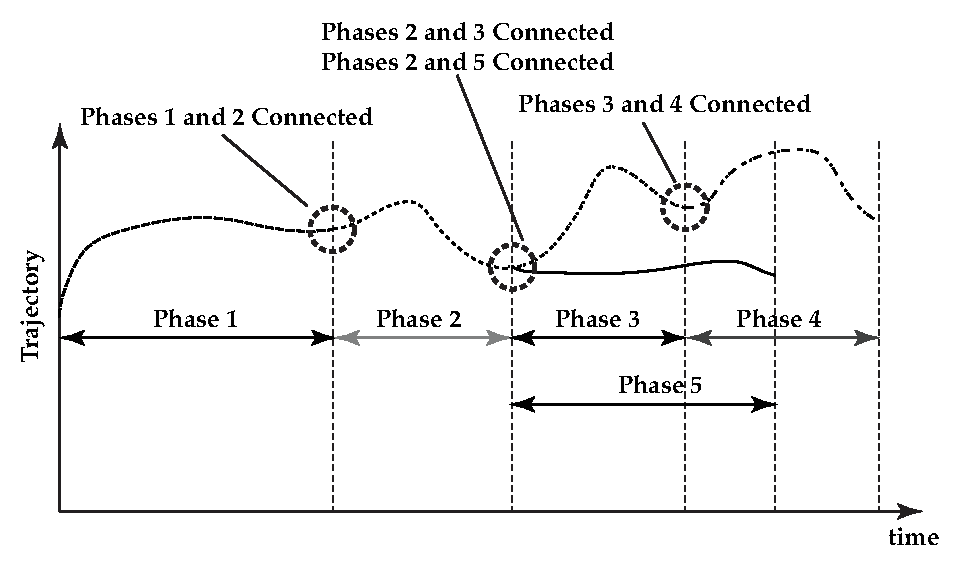
\epsfig{file=linkages.eps,height=2.8in}
  \caption{Schematic of linkages for multiple-phase optimal control problem.
    The example shown in the picture consists of five phases where the ends of
    phases 1, 2, and 3 are linked to the starts of phases 2, 3, and 4,
    respectively, while the end of phase 2 is linked to the start of phase 5.
    \label{fig: linkages}}
\end{figure}

\section{$hp$ Radau Pseudospectral Method}

In this section we describe an $hp$ version of the previously
developed Radau pseudospectral method (RPM)
\cite{Garg1,Garg2,Garg3,Patterson1}.  In order to describe the RPM,
it will be useful to modify the general optimal control problem given
in Eqs.~(\ref{general-cost})--(\ref{general-path}) as follows.  In
order to describe the method in a tractable manner, we consider only a
single phase problem (thus dropping the dependence on the superscript
$p$) and simplify the optimal control problem slightly as follows.
Determine  the state, $\bfy(t)\in\bbR^{n}$, the control
$\bfu(t)\in\bbR^{m}$, the initial time, $t_0$, and the terminal time
$t_f$ on the time interval $t\in[t_0,t_f]$ that minimize the cost
functional  
\begin{equation}\label{bolza-cost}
  \mathcal{J} = \phi(\bfy(t_0),t_0,y(t_f),t_f)
\end{equation} 
subject to the dynamic constraints
\begin{equation}\label{bolza-dyn}
  \frac{d\bfy}{dt} = \bfa(\bfy(t),\bfu(t),t), 
\end{equation} 
the inequality path constraints
\begin{equation}\label{bolza-path}
\bfc_{\min} \leq \bfc(\bfy(t),\bfu(t),t)\leq \bfc_{\max},
\end{equation} 
and the boundary conditions
\begin{equation}\label{bolza-bc}
 \bfb_{\min} \leq \bfb(\bfy(t_0),t_0,\bfy(t_f),t_f) \leq \bfb_{\min}.
\end{equation} 
The functions $\phi$, $g$, $\bfa$, $\bfc$ and $\bfb$ are defined by
the following mappings:  
\[
\begin{array}{lllll}
   \phi & : &  \bbR^{n_y} \times \bbR \times \bbR^{n_y} \times \bbR & \rightarrow & \bbR, \\
   g & : &  \bbR^{n_y} \times \bbR^{n_u} \times \bbR & \rightarrow & \bbR, \\
   \bfa & : &  \bbR^{n_y} \times \bbR^{n_u} \times \bbR & \rightarrow & \bbR^{n_y}, \\
  \bfc & : &  \bbR^{n_y} \times \bbR^{n_u} \times \bbR & \rightarrow & \bbR^{n_c}, \\
  \bfb & : &  \bbR^{n_y} \times \bbR \times \bbR^{n_y} \times \bbR & \rightarrow & \bbR^{n_b},
 \end{array}
\]
where we remind the reader that all vector functions of time are
treated as {\em row} vectors.  


Let $s\in[-1,+1]$ be a new independent variable.  The variable $t$ is
then defined in terms of $s$ as
\begin{equation}\label{stot}
  t = \frac{t_f-t_0}{2} s + \frac{t_f+t_0}{2}.  
\end{equation}
The Bolza problem of Eqs.~(\ref{bolza-cost})--(\ref{bolza-bc}) is then
defined in terms of the variable $s$ as follows.  Determine the state,
$\bfy(s)\in\bbR^{n_y}$, the control $\bfu(s)\in\bbR^{n_u}$, the initial
time, $t_0$, and the terminal time $t_f$ on the time interval
$s\in[-1,+1]$ that minimize the cost functional
\begin{equation}\label{bolza-cost-s}
  \mathcal{J} = \phi(\bfy(-1),t_0,\bfy(+1),t_f)+\frac{t_f-t_0}{2}\int_{-1}^{+1} g(\bfy(s),\bfu(s),s;t_0,t_f)\, ds
\end{equation} 
subject to the dynamic constraints
\begin{equation}\label{bolza-dyn-s}
  \frac{d\bfy}{ds} = \frac{t_f-t_0}{2}\bfa(\bfy(s),\bfu(s),s;t_0,t_f), 
\end{equation} 
the inequality path constraints
\begin{equation}\label{bolza-path-s}
\bfc_{\min} \leq \bfc(\bfy(s),\bfu(s),s;t_0,t_f)\leq \bfc_{\max},
\end{equation}
and the boundary conditions
\begin{equation}\label{bolza-bc-s}
  \bfb_{\min} \leq \bfb(\bfy(-1),t_0,\bfy(+1),t_f) \leq \bfb_{\min}. 
\end{equation}  
Suppose now that the time interval $s\in[-1,+1]$ is divided into a 
{\em mesh} consisting of $K$ {\em mesh intervals} 
$[s_{k-1},s_k],\; k=1,\ldots,K$, where  $(s_0,\ldots,s_K)$ are the
{\em mesh points}.  The mesh points have the property that
$-1=s_0<s_1<s_2<\cdots<s_K=s_f=+1$.  Next, let $\bfy^{(k)}(s)$ and
$\bfu^{(k)}(s)$ be the state and control in mesh interval $k$. The
Bolza optimal control problem of
Eqs.~(\ref{bolza-cost-s})--(\ref{bolza-bc-s}) can then written as
follows.  First, the cost functional of Eq.~(\ref{bolza-cost-s}) can
be written as 
\begin{equation}\label{bolza-cost-segmented}
  \begin{split}
 \mathcal{J} & = \phi(\bfy^{(1)}(-1),t_0,\bfy^{(K)}(+1),t_f) \\
                   &+ \frac{t_f-t_0}{2}\sum_{k=1}^K \int_{s_{k-1}}^{s_k} g(\bfy^{(k)}(\tau),\bfu^{(k)}(\tau),\tau;t_0,t_f)\, d\tau, \quad  (k=1,\ldots,K). 
  \end{split}
\end{equation}
Next, the dynamic constraints of Eq.~(\ref{bolza-dyn-s}) in mesh
interval $k$ can be written as  
\begin{equation}\label{bolza-dyn-segmented}
  \frac{d\bfy^{(k)}(s)}{ds} = \frac{t_f-t_0}{2}\bfa(\bfy^{(k)}(s),\bfu^{(k)}(s),s;t_0,t_f), \quad (k=1,\ldots,K).
\end{equation}
Furthermore, the path constraints of (\ref{bolza-path-s}) in  mesh
interval $k$ are given as
\begin{equation}\label{bolza-path-segmented}
  \bfc_{\min} \leq \bfc(\bfy^{(k)}(s),\bfu^{(k)}(s),s;t_0,t_f) \leq
  \bfc_{\max}, \quad (k=1,\ldots,K).  
\end{equation}
Finally, the boundary conditions of Eq.~(\ref{bolza-bc-s}) are given as
\begin{equation}\label{bolza-bc-segmented}
\bfb_{\min} \leq \bfb(\bfy^{(1)}(-1),t_0,\bfy^{(K)}(+1),t_f) \leq  \bfb_{\max}.  
\end{equation} 
Because the state must be continuous at each interior mesh point, it
is required that the condition $\bfy(s_k^{-})=\bfy(s_k^{+}),$ be
satisfied at the interior mesh points $(s_1,\ldots,s_{K-1})$.  

%--------------------------------------------------------------
%--------------------------------------------------------------

\section{Radau Pseudospectral Method}
%--------------------------------------------------------------

The simplified multiple-interval form of the continuous-time Bolza
optimal control problem is discretized using the previously developed
{\em Radau pseudospectral method} as described in \citeN{Garg1}.
An advantage of using the Radau scheme is that the continuity
conditions $\bfy(s_k^{-})=\bfy(s_k^{+})$ across mesh points are
particularly easy to implement.

In the Radau pseudospectral method, the state of the continuous-time
Bolza optimal control problem is approximated in each mesh interval
$k\in[1,\ldots,K]$ as 
\begin{equation}\label{state-approximation-RPM}
 \bfy^{(k)}(s)  \approx \bfY^{(k)}(s) = \sum_{j=1}^{N_k+1} \bfY_{j}^{(k)}
 \ell_{j}^{(k)}(s), \quad  \ell_{j}^{(k)}(s) = \prod_{\stackrel{l=1}{l\neq j}}^{N_k+1}\frac{s-s_{l}^{(k)}}{s_{j}^{(k)}-s_{l}^{(k)}}, 
\end{equation} 
where $s\in[-1,+1]$, $\ell_{j}^{(k)}(s),$ $j=1,\ldots,N_k+1$, is a
basis of Lagrange polynomials, $(s_1^{(k)},\ldots,s_{N_k}^{(k)})$ are the
Legendre-Gauss-Radau\cite{Abramowitz1} (LGR) collocation points
in mesh interval $k$ defined on the subinterval $s\in[s_{k-1},s_k)$, and
$s_{N_k+1}^{(k)}=s_k$ is a noncollocated point.  Differentiating
$\bfY^{(k)}(s)$ in Eq.~(\ref{state-approximation-RPM}) with respect
to $s$, we obtain
\begin{equation}\label{diff-state-approximation-RPM}
  \frac{d\bfY^{(k)}(s)}{ds} = \sum_{j=1}^{N_k+1}\bfY_{j}^{(k)}\frac{d\ell_j^{(k)}(s)}{ds}.
\end{equation}
The cost functional of Eq.~(\ref{bolza-cost-segmented}) is then
approximated using a multiple-interval LGR quadrature as  
\begin{equation}\label{RPM-cost}
  \mathcal{J} \approx \phi(\bfY_{1}^{(1)},t_0,\bfY_{N_K+1}^{(K)},t_K)  +
  \sum_{k=1}^{K} \sum_{j=1}^{N_k}  \frac{t_f-t_0}{2} 
  w_{j}^{(k)} g(\bfY_{j}^{(k)},\bfU_{j}^{(k)},s_{j}^{(k)};t_0,t_f),
\end{equation}
where $w_j^{(k)},\;j=1,\ldots,N_k$ are the LGR quadrature
weights\cite{Abramowitz1} in mesh interval $k\in[1,\ldots,K]$ defined 
on the interval $s\in[s_{k-1},s_k)$, $\bfU_i^{(k)},$ $i=1,\ldots,N_k$,
are the approximations of  the control at the $N_k$ LGR points in mesh
interval $k\in[1,\ldots,K]$, $\bfY_1^{(1)}$ is the approximation of
$\bfy(s_0=-1)$, and $\bfY_{N_K+1}^{(K)}$ is the approximation of $\bfy(s_K=+1)$.
Collocating the dynamics of Eq.~(\ref{bolza-dyn-segmented}) at the
$N_k$ LGR points using Eq.~(\ref{diff-state-approximation-RPM}), we have
\begin{equation}\label{RPM-collocation-conditions}
  \sum_{j=1}^{N_k+1}D_{ij}^{(k)} \bfY_j^{(k)} - \frac{t_f-t_0}{2} \bfa(\bfY_i^{(k)},\bfU_i^{(k)},s_i^{(k)};t_0,t_f) = \bfzero, \quad (i=1,\ldots,N_k).  
\end{equation}
where $t_i^{(k)}$ are obtained from $s_k^{(k)}$ using Eq.~(\ref{stot})
and 
\begin{equation}\label{Radau-differentiation-matrix}
  D_{ij}^{(k)} = \left[\frac{d\ell_j^{(k)}(s)}{ds}\right]_{s_i^{(k)}}, \quad
   (i=1,\ldots,N_k, \quad j=1,\ldots,N_k+1,\quad k=1,\ldots,K),
\end{equation}
is the $N_k\times (N_k+1)$ {\em Radau pseudospectral differentiation
matrix}\cite{Garg1} in mesh interval $k\in[1,\ldots,K]$. 
Next, the path constraints of Eq.~(\ref{bolza-path-segmented})
in mesh interval $k\in[1,\ldots,K]$ are enforced at the $N_k$ LGR points as   
\begin{equation}\label{RPM-path-constraint}
  \bfc_{\min} \leq  \bfc(\bfY_{i}^{(k)},\bfU_{i}^{(k)},s_{i}^{(k)};t_0,t_f) \leq \bfc_{\max}, \quad (i=1,\ldots,N_k).
\end{equation}
Furthermore, the  boundary conditions of
Eq.~(\ref{bolza-bc-segmented}) are approximated as
\begin{equation} \label{RPM-bcs} 
 \bfb_{\min} \leq \bfb(\bfY_{1}^{(1)},t_0,\bfY_{N_K+1}^{(K)},t_f)  \leq \bfb_{\max}.  
\end{equation} 
It is noted that continuity in the state at the interior mesh points 
$k\in[1,\ldots,K-1]$ is enforced via the condition 
\begin{equation} \label{RPM-continuity}
\bfY_{N_k+1}^{(k)} = \bfY_1^{(k+1)} , \quad (k=1,\ldots,K-1),
\end{equation}
where we note that the {\em same} variable is used for both
$\bfY_{N_k+1}^{(k)}$ and $\bfY_1^{(k+1)}$.  Hence, the constraint of
Eq.~(\ref{RPM-continuity}) is eliminated from the problem because it
is taken into account explicitly.  The NLP that arises from the Radau
pseudospectral approximation is then to minimize the cost function of 
Eq.~(\ref{RPM-cost}) subject to the algebraic constraints of
Eqs.~(\ref{RPM-collocation-conditions})--(\ref{RPM-bcs}).

\begin{figure}
 \centering
 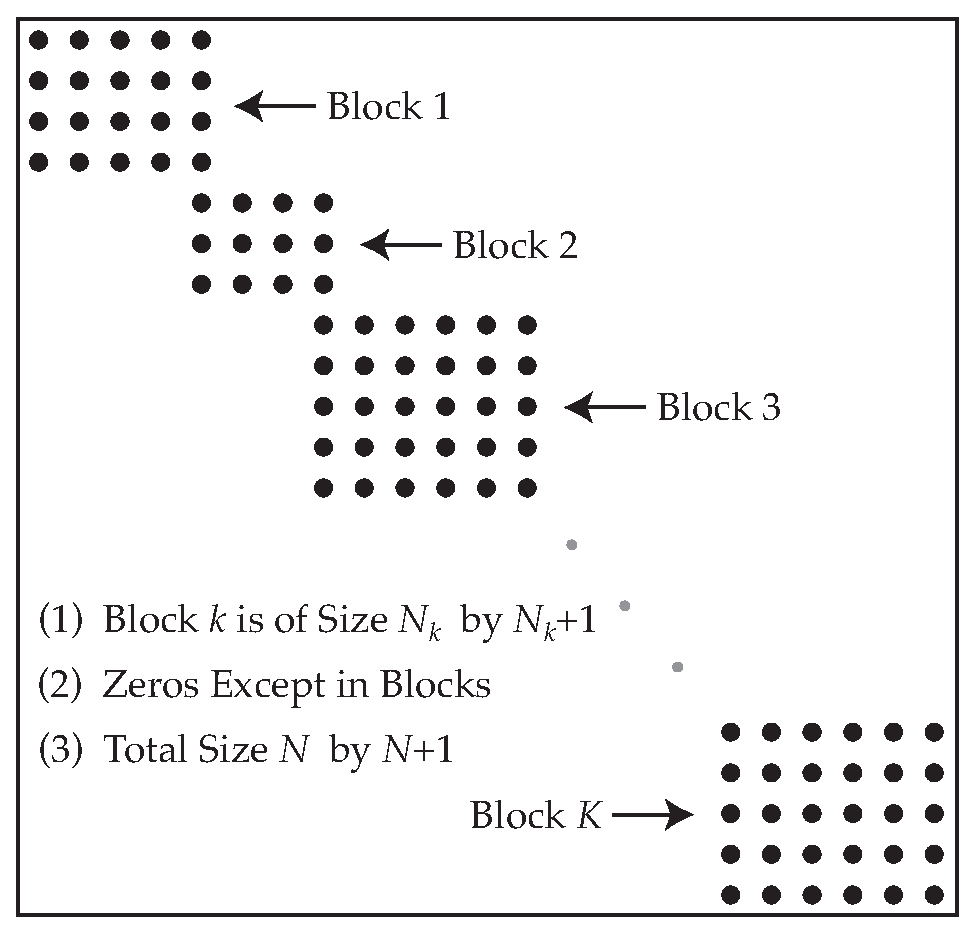
\epsfig{file=RPMDmatrixStructure.eps,height=2in}
 \caption{Structure of Composite Radau Pseudospectral Differentiation
   Matrix Where the Mesh Consists of $K$ Mesh Intervals.\label{fig:RPMDmatrix}}
\end{figure}

\bibliographystyle{acmsmall}
\bibliography{bibliography}

\end{document}

\section{$hp$--Adaptive Radau Pseudospectral Method}

In this section we provide a detailed description of the
discretization of a multiple-phase optimal control problem via the 
GPM.  For completeness, we restate some of the basic equations that have been previously
developed for the GPM \cite{Benson1,Benson2,Huntington0}. 

Let $p\in[1,\ldots,P]$ be a particular phase of an optimal control
problem and let $(\cdot)^{(p)}$ denote information in the $p^{th}$
phase.  For every phase of the problem, consider now the following
transformation of the independent variable, $t$, to the variable
$\tau\in[-1,1]$:\footnote{For simplicity with the remainder of this
  section, superscript ``$(p)$'' denoting the phase number will be
  suppressed unless it is needed to distinguish between phases.}
\begin{equation}\label{time_map}
  t^{(p)} = \frac{t_f^{(p)}-t_0^{(p)}}{2} \tau^{(p)} + \frac{t_f^{(p)}+t_0^{(p)}}{2}
\end{equation}
Furthermore, suppose we choose the collocation points in
each phase to be the set of {\em Legendre-Gauss} (LG) points, 
$(\tau_1,\ldots,\tau_{N^{(p)}})$, which are the roots of the
$N^{th}$-degree Legendre polynomial, $P_N(\tau)$, given
as\footnote{The Legendre-Gauss (LG) points are
  conveniently obtained by computing the eigenvalues of
  the$N\times N$ {\em Jacobi matrix} as is done in the
  pseudospectral differentiation matrix suite \cite{Weideman1}.} 
\begin{equation}
P_{N} = \frac{1}{2^{N}N!}\frac{d^{N}}{d\tau^{N}}\left\{\left[\tau^2-1\right]^N\right\}
\end{equation}
Corresponding to the LG points are the LG {\em weights} which are computed as
\begin{equation} \label{LG weights}
  w_i = \frac{2}{\left(1-\tau_i^2\right)\left[P_{N}^{\prime}\right]^2}, \qquad (i=1,\ldots,N)
\end{equation}
Finally, the {\em discretization points} used in the GPM are the LG
points plus the points $\tau_0=-1$ and $\tau_{N+1}=1$ (thus
resulting in a complete set of points
$(\tau_0,\ldots,\tau_{N+1})$. 

The discretization in each phase $p=[1,\ldots,P]$ of the problem can
then be stated in terms of the independent variable $\tau$ as
follows.  First, the state is approximated using a  basis of
$N+1$ Lagrange interpolating polynomials,
$L_i(\tau),\;(i=0,\ldots,N)$, 
\begin{equation} \label{state approximation gauss}
  \bfx(\tau) \approx \bfX(\tau) = \sum_{i=0}^{N}
  \bfX(\tau_i) L_i(\tau)
\end{equation}
where $L_i(\tau)\;(i=0,\ldots,N)$ are defined as
\begin{equation}
  L_i(\tau)  = \displaystyle \prod_{j=0,j\neq i}^{N}
  \frac{\tau-\tau_j}{\tau_i-\tau_j}
  \label{lagrange for state}
\end{equation}
It is known that the Lagrange polynomials
$L_i(\tau)\;(i=0,\ldots,N)$ satisfy the so called
{\em isolation property} 
\begin{equation}
  L_i(\tau_j) = \left\{\begin{array}{ccc} 1 & , & i=j \\ 0 & , &
      i\neq j \end{array} \right.
  \label{lagrange state property}
\end{equation}
The continuous cost functional of Eq.~(\ref{general cost}) is then
approximated using the values of the state, control, and time at the
LG points via a Gauss quadrature \cite{Davis1} as 
\begin{equation}\label{diff_dis_cost}
  \begin{split}
    J & = \sum_{p=1}^{P} \Phi^{(p)}(\bfX_0^{(p)},t_0^{(p)},\bfX_f^{(p)},t_f^{(p)}) \\ &
    + \sum_{p=1}^{P} \displaystyle\frac{t_f^{(p)}-t_0^{(p)}}{2}\sum_{k=1}^{N^{(p)}} w_k^{(p)}\mcL^{(p)}(\bfX_k^{(p)},\bfU_k^{(p)},\tau_k^{(p)};\bfq^{(p)},t_0^{(p)},t_f^{(p)})
\end{split}
\end{equation}
Next, differentiating the expression in 
Eq.~(\ref{state approximation gauss}) with respect to $\tau$ gives 
\begin{equation}
  \frac{d\bfX}{d\tau} \approx \sum_{i=0}^{N} \bfX(\tau_i)
  \frac{d{L}_i(\tau)}{d\tau} \label{derivative state approximation}
\end{equation}
The derivative of each Lagrange polynomial at the LG points can be
represented compactly in the form of a {\em differentiation matrix}, $\bfD\in\mathbb{R}^{N\times N+1}$ as
\begin{equation}
  \bfD_{ki} = \dot L_i(\tau_k) = \sum_{l=0}^{N} \frac{\displaystyle
    \prod_{j = 0,j \not= i,l}^{N} \left(\tau_k - \tau_j\right)}{\displaystyle
    \prod_{j = 0,j \not= i}^{N} \left(\tau_i - \tau_j\right)}
\end{equation}
where $k = 1,\ldots,N$ and $i = 0,\ldots,N$.  The dynamic constraint of
Eq.~(\ref{general dynamics}) is then  transcribed into algebraic
constraints in each phase $p=[1,\ldots,P]$ of the problem as
\begin{equation}\label{diff_dis_dyn}
    \sum_{i=0}^N \bfD_{ki}
    \bfX_i - \displaystyle\frac{t_f-t_0}{2}
    \textbf{f}(\bfX_k,\bfU_k,\tau_k;\bfq,t_0,t_f) = \textbf{0} \quad
    (k = 1,\ldots,N)
\end{equation}
where $\bfX_k \equiv
\bfX(\tau_k)\in\mathbb{R}^{n}$ and $\bfU_k
\equiv \bfU(\tau_k)\in\mathbb{R}^{m}$
$(k=1,\ldots,N$). Next, define an additional variable
$\bfX_f\equiv\bfX_{N+1}\equiv\bfX(\tau_f)$
as
\begin{eqnarray}
    \bfX_0 & = & \bfX(\tau_0) \\
    \bfX_{N+1} & = &   \bfX_0 + \displaystyle\frac{t_f-t_0}{2}\sum_{k=1}^N w_k
  \textbf{f}(\bfX_k,\bfU_k,\tau_k;\bfq,t_0,t_f) \label{gauss quadrature of xf}
\end{eqnarray}
It is noted that, because we have introduced an additional variable,
Eq.~(\ref{gauss quadrature of xf}) is an additional constraint in the
discretization (in order to maintain the same number of degrees of
freedom).  Now, because Eq.~(\ref{gauss quadrature of xf}) is a
function of the right-hand side of the differential equation at each
LG point, Eq.~(\ref{diff_dis_dyn}) can be used to solve for
$\textbf{f}$ and the result can be substituted into 
Eq.~(\ref{gauss quadrature of xf}).  The result of this substitution
transforms Eq.~(\ref{gauss quadrature of xf}) into a linear equation
given as
\begin{equation} \label{gauss quadrature of xf linear}
    \bfX_{N+1} - \bfX_0 - \sum_{i=0}^{N} \sum_{k=1}^{N} 
    w_k \bfD_{ki} \bfX_i = \bfzero
\end{equation}
Because it is linear, Eq.~(\ref{gauss quadrature of xf linear}) is
implemented [as opposed to Eq.~(\ref{gauss quadrature of xf})].
Similarly, the path constraints of Eq.~(\ref{general path}) are
discretized at the LG points as 
\begin{equation}\label{diff_dis_path}
  \bfC_{\min}\leq\textbf{C}(\bfX_k,\bfU_k,\tau_k;t_0,\bfq,t_f)\leq\bfC_{\max}\quad (k = 1,\ldots,N)
\end{equation}
Furthermore, the boundary conditions of  Eq.~(\ref{general boundary
  conditions}) are expressed as 
\begin{equation}\label{diff_dis_bound}
  \bfphi_{\min} \leq \boldsymbol{\phi}(\bfX_0,t_0,\bfX_{N+1},t_f) \leq\bfphi_{\max}
\end{equation}
Finally, the linkage constraints are mapped using the values at the
termini and start, respectively, of the phase pairs
$(p_l,p_r)\in[1,\ldots,P]$ ($l,r=[1,\ldots,P]$) as 
\begin{equation}\label{dis_linkages}
  \bfL_{\min}^{(s)} \leq\bfL^{(s)}(\bfX_{N+1}^{(p_l^s)},t_f^{(p_l^s)};\bfq^{(p_l^s)},\bfX_0^{(p_u^s)},t_0^{(p_u^s)};\bfq^{(p_u^s)})
  \leq \bfL_{\max}^{(s)}, \; \left\{\begin{array}{lcl} p_l,p_u & \in& [1,\ldots,P] \\ s & = & 1,\ldots,L\end{array} \right.
\end{equation}


\section{Algorithm for Solving Multiple-Phase Optimal Control Problems
  Using the Gauss Pseudospectral Method} \label{nlp_mapping}

In this section we provide the algorithm for mapping of the
multiple-phase GPM to an NLP in standard form.  As mentioned in the
introduction, we note that the approach described in this section is a
generalization of many custom (non-reusable)
MATLAB programs that have been developed by the
authors or MATLAB programs co-developed by the
authors and their colleagues \cite{Rao7,Benson1,Huntington0,Huntington1,Huntington2,Huntington3,Huntington5}.
It is noted that the algorithm described is a formalization of 
an extensive amount of programming experience.

In general, an NLP has the following standard form.  Minimize the cost
function
\begin{equation}\label{general nlp cost}
  f(\bfZ)
\end{equation}
subject to the algebraic equality and inequality constraints
\begin{equation}\label{general nlp constraints}
  \begin{array}{lcccr}
    \bfZ_{\min} & \leq & \bfZ & \leq & \bfZ_{\max} \\
    & & \bfc_E(\bfZ) & = & \bfzero \\
    \bfc_{I,\min} & \leq & \bfc_I(\bfZ) & \leq & \bfc_{I,\max}
  \end{array}
\end{equation}

It is important to note in Eqs.~(\ref{general nlp cost}) and
(\ref{general nlp constraints}) that the column vector
$\bfz\in\mathbb{R}^{n_z}$ contains the NLP decision variables for the
{\em entire} problem.  Similar, $\bfc(\bfz)$ is a column vector of
constraints for the {\em entire} problem.  Finally the subscripts
``$E$'' and ``$I$'' correspond, respectively, to the {\em equality}
and the {\em inequality} constraints.  Recalling that the entire problem consists
of $P$ phases and denoting the decision vector within a given 
phase $p\in[1,\ldots,P]$ by $\bfz$, the complete vector of decision
variables is a concatenation of the decision variables in each phase
of the problem, \ie  
\begin{equation}\label{total optimization vector 1}
  \bfZ = \left[\begin{array}{c} \bfz^{(1)} \\ \vdots \\ \bfz^{(P)} \end{array} \right]
\end{equation}
In order to make the algorithm somewhat more manageable, the
constraints are rearranged such that the constraints in each phase are
a concatenation of the equality constraints and inequality constraints
in the  phase, \ie 
\begin{equation}
  \bfc^{(p)} = \left[\begin{array}{c} \bfc_E^{(p)} \\ \bfc_I^{(p)} \end{array} \right]
\end{equation}
where $\bfc$ is the subvector of constraints in phase $p=[1,\ldots,P]$.  Finally, appended to the phase constraints are the {\em linkage} constraints, denoted $\bfc_{L}$.  The total constraint vector is then given as
\begin{equation}
  \bfc = \left[\begin{array}{c} \bfc^{(1)} \\ \vdots \\ \bfc^{(P)} \\ \bfc_{L} \end{array} \right]
\end{equation}

\subsection{Mapping of Decision Variables in a Single Phase}

We now proceed to describe the mapping of the optimization vector
within a particular phase $p\in[1,\ldots,P]$ to the values of the
state, control, time, and static parameters.  In order to make it
easier to follow the details, the superscript $(\cdot)^{(p)}$
(denoting the phase number) is for the most part  suppressed.   

The total vector of optimization variables
$\bfz\in\bbR^{n_x(N+2)+n_uN+n_q+2}$ in a particular phase
$p=[1,\ldots,P]$ is given as 
\begin{equation}
  \bfz^{(p)} \equiv \bfz = \left[
    \begin{array}{c}
      \bfz_x \\
      \bfz_u \\
      \bfq \\
      t_0 \\
      t_f
    \end{array} \right], \qquad (p=1,\ldots,P)
\end{equation}
where $\bfz_x$ is the vector of variables associated with the values
of the state at the discretization points, $\bfz_u$ is the vector of
variables associated with the values of the control at the LG points,
$\bfq$ is the vector of static optimization parameters, $t_0$ is the
initial time, and $t_f$ is the terminal time.  The vector $\bfz_x$ is
given as 
\begin{equation}
  \bfz_x = 
  \left[\begin{array}{c}
      \bfchi_1 \\ \vdots \\ \bfchi_{n_x}
      \end{array}
    \right]
\end{equation}
where the column vectors $\bfchi_j,\;(j=1,\ldots,n_x)$ are given as
\begin{equation}
  \bfchi_j = \left[\begin{array}{c} x_{j1} \\ \vdots \\ x_{j,(N+2)}\end{array} \right], \qquad (j=1,\ldots,n_x)
\end{equation}
and $x_{jk},\;(j=1,\ldots,n_x;k=1,\ldots,N+2)$ is the value of the
$j^{th}$component of the state at the $k^{th}$ discretization point.
Next, the vector $\bfz_u$ is given as 
\begin{equation}
  \bfz_u = 
  \left[\begin{array}{c}
      \bfsigma_1 \\ \vdots \\ \bfsigma_{n_u}
      \end{array}
    \right]
\end{equation}
where the column vectors $\bfsigma_j,\;(j=1,\ldots,n_u)$ are given as
\begin{equation}
  \bfsigma_j = \left[\begin{array}{c} u_{j1} \\ \vdots \\ u_{j,N}\end{array} \right], \qquad (j=1,\ldots,n_u)
\end{equation}
and $u_{jk},\;(j=1,\ldots,n_u;k=1,\ldots,N)$ is the value of the
$j^{th}$ component of the control at the $k^{th}$ collocation (LG)
point.  For use in vectorized operations in
MATLAB \cite{Mathworks1}, it is convenient to reshape the vectors
$\bfz_x$ and $\bfz_u$ into matrices $\bfY_x\in\bbR^{(N+2)\times n_x}$
and $\bfY_x\in\bbR^{N\times n_u}$ whose rows contain a single vector
value of the state and control, respectively.  First,  
$\bfY_x$ is obtained from $\bfz_x$ as
\begin{equation}
  \bfY_x = \mathbf{reshape}(\bfz_x,N+2,n_x)
\end{equation}
where $\mathbf{reshape}$ is a pseudo-coded version of the
MATLAB ``reshape'' command.  The vector $\bfz_x$
can be re-acquired from $\bfY_x$ as 
\begin{equation}
  \bfz_x = \bfY_x(:)
\end{equation}
where ``:'' is a pseudo-coded version of the
MATLAB\cite{Mathworks1} column-stacking
operator.  Next, $\bfY_u$ is obtained from $\bfz_u$ as 
\begin{equation}
  \bfY_u = \mathbf{reshape}(\bfz_u,N,n_u)
\end{equation}
The vector $\bfz_u$ can be re-acquired from $\bfY_u$ as
\begin{equation}
  \bfz_u = \bfY_u(:)
\end{equation}

\subsection{Construction of Total Vector of Decision Variables}

To construct the total vector of NLP decision variables, the process
described in the previous subsection is repeated for all phases
$p=[1,\ldots,P]$.  In other words, we construct the vector $\bfz$ by
stacking the variables $\bfz^{(p)}$ using Eq.~(\ref{total optimization
  vector 1}).   

\subsection{Construction of Constraint Vector within a Single Phase}

Next, the algorithm for constructing the column vector of all NLP
constraints within a given phase is described.  The constraints within
a single phase are obtained by stacking the collocated dynamic
constraints, the collocated path constraints, and the boundary
conditions.\footnote{It is noted that the collocated dynamic
  constraints are {\em equality} constraints while the path
  constraints and boundary conditions are {\em inequality}
  constraints.}  The vector of constraints within a single phase can
then be written as 
\begin{equation}
  \bfc(\bfz) = \left[\begin{array}{c} \bfc_E(\bfz) \\ \bfc_I(\bfz) \end{array} \right]
\end{equation}
where, as before, the subscripts ``$E$'' and ``$I$'' correspond to
{\em equality} and {\em inequality} constraints, respectively.  A
relatively straightforward way to map the equality constraints to a
single column vector is as follows.  First, suppose we define the {\em
  defect constraints}, $\bfdelta_k,\;k=1,\ldots,N$, as 
\begin{eqnarray}\label{ode defects}
  \bfdelta_k  & = & \sum_{i=0}^{N} \bfD_{ki}\bfX_i - \frac{t_f-t_0}{2} \bff(\bfX_k,\bfU_k,t_k;\bfq), \qquad (k=1,\ldots,N) \\
\bfdelta_{N+1} & = &     \bfX_{N+1} - \bfX_0 - \sum_{i=0}^{N} \sum_{k=1}^{N}   w_k \bfD_{ki} \bfX_i = \bfzero
\end{eqnarray}
where we have assumed that $\bff(\bfX_k,\bfU_k,t_k;\bfq)$ is a {\em row}
vector of length $n$.  Then we can define the matrix $\bfDelta$ as 
\begin{equation}
  \bfDelta = \left[\begin{array}{c} \bfdelta_1 \\ \vdots \\
 \bfdelta_{N+1} \end{array} \right]
\end{equation}
It turns out that $\bfDelta$ can be computed as
\begin{equation}
  \bfDelta =
  \left[\begin{array}{c}
      \bfD \bfY_x(1:N+1,:)-\frac{t_f-t_0}{2}\bfF \\
      \bfY_x(\textrm{end},:)-\bfY_x(1,:)-\bfw^T \bfD \bfY(1:N+1,:)
    \end{array} \right]
\end{equation}
where $\bfw$ is a column vector of LG weights, the notation ``$1:N+1$''
is a pseudo-code for the first $N+1$ rows of the matrix $\bfY_x$, and
$\bfF$ is a vectorized evaluation of the right-hand sides of the
differential equations at the LG (collocation) points, \ie 
\begin{equation}\label{GPM NLP F}
  \begin{split}
    \bfF & = \left[\begin{array}{c} \bff(\bfX_1,\bfU_1,t_1;\bfq) \\ \vdots \\ \bff(\bfX_{N},\bfU_{N},t_{N};\bfq)
\end{array} \right] \\ \\
& \equiv \bfF(\bfY_x(2:N+1,:),\bfY_u,\bft(2:N+1);\bfq)
\end{split}
\end{equation}
where the column vector $\bft\in\bbR^{N+2}$ is given as
\begin{equation}
  \bft = \left[\begin{array}{c} t_0 \\ t_1 \\ \vdots \\ t_{N+1} \end{array} \right]
\end{equation}
The matrix $\bfDelta$ can then be isomorphically mapped to the column
vector of equality constraints  $\bfc_{E}$ using a pseudo-coded
version of the MATLAB \cite{Mathworks1}
column-stacking operator ``:'' as 
\begin{equation}
  \bfc_{E} = \bfDelta(:)
\end{equation}
Next, let $\bfH_{C}$ be the matrix that arises from the evaluation of
the path constraints at all of the LG points.  Then $\bfH$ is given as 
\begin{equation} \label{path constraint matrix}
  \bfH_{C} = \left[\begin{array}{c} \bfC(\bfX_1,\bfU_1,t_1;\bfq) \\ \vdots \\ \bfC(\bfX_{N},\bfU_{N},t_{N};\bfq)
\end{array} \right] \equiv \bfC(\bfY_x(2:N+1,:),\bfY_u,\bft;\bfq)
\end{equation}
Also, let $\bfH_{\phi}$ be the vector that arises from the evaluation
of the boundary conditions.  Noting that the boundary conditions are
functions of only the state and time at the endpoints of the phase, we
have 
\begin{equation}
  \bfH_{\phi} = \bfphi(\bfY_x(1,:),t_0,\bfY_x(\textrm{end},:),t_f)
\end{equation}
where it is noted that $\bfY_x(1,:)=\bfX_0$ and
$\bfY_x(\textrm{end},:)=\bfX_f$, respectively.  The inequality
constraint vector is then given as 
\begin{equation}
  \bfc_{I} = \left[\begin{array}{c} \bfH_C(:) \\ \bfH_{\phi} \end{array}\right]
\end{equation}
where we once again note the use of the MATLAB \cite{Mathworks1}
column-stacking operator ``:'' to isomorphically map the matrix of
path constraints to a column vector of length $n_cN$.  

\subsection{Construction of Linkage Constraint Vector}

The vector of linkage constraints is obtained by using the values of the
state and time at the terminus and start of each pair that is to be
linked.  We can write the evaluation of the $s^{th}$ set of linkage
constraints as follows: 
\begin{equation}\label{linkage for set S}
  \begin{array}{c}
    t_f^{(p_l^{(s)})}- t_0^{(p_r^{(s)})} \\
  \bfS^{(s)}(\bfY_x^{(p_l^{(s)})}(\textrm{end},:),\bfq^{(p_l^{(s)})},\bfY_x^{(p_r^{(s)})}(1,:),\bfq^{(p_r^{(s)})})
  \end{array}, \qquad
  \left\{\begin{array}{lcl} p_l,p_r & \in& [1,\ldots,P] \\ s & = &1,\ldots,L\end{array} \right.
\end{equation}
It is noted that the linkage conditions in Eq.~(\ref{linkage for set S})
have been separated into those that link the independent variable (\ie
time) between phases and those that link the state and parameters
between phases.  The reason for this separation is that the linkage of
the independent variable is a {\em linear} constraint and thus has a
structure that can be taken advantage of when implementing the NLP in
software.   

\section{Construction of Total Vector of Constraints}

The total vector of constraints for all phases and the linkage
constraints is then given as 
\begin{equation}\label{general constraints}
  \bfc(\bfZ) = \left\{
    \begin{array}{c}
      \left[
        \begin{array}{c}
          \bfDelta^{(1)}(:) \\
          \bfH_C^{(1)}(:) \\ \bfH_{\phi}^{(1)}
        \end{array}
      \right] \\ \\
      \vdots \\ \\
      \left[
        \begin{array}{c}
          \bfDelta^{(P)}(:) \\
          \bfH_C^{(P)}(:) \\ \bfH^{(P)}_{\phi}
        \end{array}
      \right] \\ \\
      \left[ \begin{array}{c}
          t_f^{(p_l^{(1)})}- t_0^{(p_r^{(1)})} \\
          \bfS^{(1)}(\bfY_x^{(p_l^{(1)})}(\textrm{end},:),\bfq^{(p_l^{(1)})},\bfY_x^{(p_r^{(1)})}(1,:),\bfq^{(p_r^{(1)})})
        \end{array} \right] \\ \\
      \vdots \\ \\
      \left[ \begin{array}{c}
    t_f^{(p_l^{(L)})}- t_0^{(p_r^{(L)})} \\
  \bfS^{(L)}(\bfY_x^{(p_l^{(L)})}(\textrm{end},:),\bfq^{(p_l^{(L)})},\bfY_x^{(p_r^{(L)})}(1,:),\bfq^{(p_r^{(L)})})
  \end{array} \right]
    \end{array} \right\}
\end{equation}

\section{Structure of Gauss Pseudospectral NLP Sparsity Pattern} \label{sect: sparsity}

As it turns out, the NLP described in the previous section has an
extremely well-defined structure that can be taken advantage of in a
software implementation.  First, the constraint Jacobian,
$\partial\bfc/\partial\bfz$, is {\em sparse}.   A graphical
representation of the structure of a single phase of the constraint
Jacobian is shown in Fig.~\ref{fig: sparsity phase}.  The sparsity
pattern for a given phase $p\in[1,\ldots,P]$ is divided into rows and
columns such that the rows correspond to the phase constraints while the
columns correspond to the phase variables.  Furthermore, the rows in 
Fig.~\ref{fig: sparsity phase} contain the derivatives of the defect
constraints, path constraints, and event constraints with respect to
each value of the state, control, initial and terminal times, and the
static parameters. The derivatives of the defect constraints are
divided into a set of main diagonal blocks and off-diagonal blocks.
The main diagonal blocks are the derivatives of the $i^{th}$ set of
defect constraints (\ie those associated with the $i^{th}$ state) with
respect to the values of the $i^{th}$ state at the discretization
points.  The  off-diagonal blocks of the derivatives of the defect
constraints are the derivatives with respect to the values of the
$j^{th}$ state (where $j\neq i)$ and the $k^{th}$ control (in that
order column-wise).  Finally, the columns that lie to the right of 
those associated with the control are the derivatives with respect to
the initial time, $t_0$, the terminal time, $t_f$, and the static
parameters $\bfq$, respectively.  The rows of the phase sparsity that
lie below those associated with the defect constraints are the
derivatives of the path constraints and contain the derivatives with
respect to the values of the state, control, initial and terminal
times, and static parameters.  Finally, the rows that lie below those
associated with the path constraints contain the derivatives of the
event constraints.  It is seen that the event constraint derivatives 
are nonzero only with respect to the initial state and terminal state,
the initial and terminal time, and the static parameters.  

Using the phase sparsity given in Fig.~\ref{fig: sparsity phase}, the
complete sparsity pattern for a multiple-phase problem is shown in 
Fig.~\ref{fig: sparsity}.  It is seen that the complete sparsity
pattern is block-diagonal concatenation of the sparsity pattern in
each phase, where the variables in each phase are non-overlapping with
the exception of the linkage constraints .  With regard to the linkage
constraint derivatives, the overlap in variables between phases is
confined to variables at the terminus and start of the pair of phases
to be linked.  

\begin{figure}[h]
  \centering
  \epsfig{file=sparsity_phase.eps,height=4.8in}
  \caption{Structure of Single Phase of Constraint Jacobian of discretization of Multiple-Phase Gauss Pseudospectral Method.
\label{fig: sparsity phase}}
\end{figure}

\begin{figure}[h]
  \centering
  \epsfig{file=sparsity.eps,height=3.5in}
  \caption{Structure of Entire Sparsity Pattern for discretization of the Multiple-Phase Gauss Pseudospectral Method.  Each Phase Has Nonzeros as Given in Fig.~\ref{fig: sparsity phase}.
\label{fig: sparsity}}
\end{figure}

\section{Lagrange Multipliers of NLP and Costate Mapping} 
\label{sect: costates}

Each constraint in the NLP has a corresponding Lagrange multiplier.
Suppose we let $\tilde{\bfLambda}_k^{(p)},\;(k=1,\ldots,N)$ and
$\tilde{\bfLambda}_f^{(p)}$ be the Lagrange multipliers associated
with the discretized dynamic constraints of Eq.~(\ref{diff_dis_dyn})
and the quadrature constraint of Eq.~(\ref{gauss quadrature of xf linear}),
respectively, in each phase $p=[1,\ldots,P]$ of the optimal control
problem.  Furthermore, let
$\tilde{\boldsymbol{\mu}}_k,\;(k=1,\ldots,N)$ be the Lagrange
multipliers associated with the discretized path constraints of
Eq.~(\ref{diff_dis_path}).  Finally, let 
$\tilde{\boldsymbol{\nu}}$ be the Lagrange multiplier associated with
the discretized boundary conditions of Eq.~(\ref{diff_dis_bound}).
Then it has been shown \cite{Benson1,Benson2,Huntington0} that the
costate (\ie the adjoint) of the continuous-time optimal control
problem is related to the Lagrange multipliers 
$\tilde{\bfLambda}_k,\;(k=1,\ldots,N)$ and $\tilde{\bfLambda}_f$ as
\begin{equation}\label{costate equivalence}
  \begin{array}{lcl}
    \bfLambda(t_f) & = & \tilde\bfLambda_f \vspace{6pt} \\
    \bfLambda_k & = &  \tilde{\bfLambda}_k/w_k \vspace{6pt} \\
    \bfLambda(t_0) & = & (1+\alpha)\bfLambda(t_f) - \displaystyle \sum_{i=1}^{N} D_{i0} \tilde{\bfLambda}_i \vspace{6pt} \\
    \bfmu_k & = & \displaystyle\frac{2}{t_f-t_0}\frac{\tilde{\bfmu}_k}{w_k} \vspace{6pt} \\
    \bfnu & = & \tilde{\bfnu} \vspace{6pt} \\
    \alpha & = & \displaystyle \sum_{i=1}^N w_i D_{i0}
  \end{array}
\end{equation}
The NLP described in Section \ref{nlp_mapping} has a dual solution
that includes the Lagrange multipliers for each category of
discretized constraints.  In particular, suppose we let $\bfGamma$ be
the vector of Lagrange multipliers associated with the differential
dynamic constraints and the quadrature constraints.  Then, because the
dynamics are discretized at $N$ Legendre-Gauss points, we know that 
$\bfGamma\in\bbR^{n_x(N+1)}$ (\ie we have $n_xN$ multipliers for the
discretized dynamic constraints and another $N$ multipliers for the
quadrature constraints.  The column vector $\bfGamma$ can be
isomorphically mapped to a matrix of size $(N+1)\times n_x$ via a
pseudo-coded version of the MATLAB \cite{Mathworks1} command {\bf reshape} \cite{Mathworks1} as 
\begin{equation}
  \tilde{\bfM} = \textbf{reshape}(\bfGamma,N+1,n_x) =
  \left[
    \begin{array}{c}
      \tilde{\bfLambda}_1 \\ \tilde{\bfLambda}_2 \\ \vdots \\ \tilde{\bfLambda}_{N+1}
    \end{array}
    \right]
\end{equation}
where $\tilde{\bfLambda}_i,\;(i=1,\ldots,N+1)$ are row vectors.  Next,
we can construct a diagonal matrix $\bfW$ that contains the
reciprocals of the Gauss weights as 
\begin{equation}
  \bfW = \textbf{diag}(1/w_1,\ldots,1/w_{N})
\end{equation}
The costate estimate given in Eq.~(\ref{costate equivalence}) can then
be obtained at the Legendre-Gauss points as 
\begin{equation}
  \bfM = \bfW\tilde{\bfM}(1:\textrm{end}-1,:)
\end{equation}
In addition, the costate estimate at the {\em initial time} in phase
$p=[1,\ldots,P]$ is computed as 
\begin{equation}
  \bfLambda(t_0) = (1+\bfw^T\bfD(:,1))\tilde{\bfLambda}_f-\textbf{sum}(\textbf{repmat}(\bfD(:,1),1,n_x)\textbf{.}\bfM(1:\textrm{end}-1,:),1)
\end{equation}
where ``\textbf{.}'' denotes element-by-element multiplication and we
have used pseudo-coded versions of the MATLAB  commands {\bf repmat} and {\bf sum} (and, 
by virtue of the last argument being unity, the sum is taken along the
columns).  We can then augment the initial costate to the matrix
$\bfM$ to obtain the complete matrix of costates as 
\begin{equation}
  \bfM_a =
  \left[
    \begin{array}{c}
      \bfLambda_0 \\ \bfLambda_1 \\ \bfLambda_2 \\ \vdots \\ \bfLambda_{N+1}
    \end{array}
    \right]
\end{equation}

\section{Separation of Constant and Non-Constant Derivatives in Constraint Jacobian}

A unique feature of the {\em SNOPTA} interface of the NLP solver SNOPT
\cite{Gill2} is that SNOPTA allows the user to separate the constant
derivatives from the non-constant derivatives.  This feature is
described in the SNOPT 7 manual \cite{Gill1}  but is repeated here in the context of the
Gauss pseudospectral method.  First, consider a problem such that each
function (constraint or objective) can be written in the form 
\begin{equation}
  F_i(\bfx) = f_i(\bfx) + \sum_{j=1}^{n} A_{ij} \bfx_j
\end{equation}
$f_i(\bfx)$ is a nonlinear function, $n$ is the total number of
optimization (decision) variables, $\bfx\in\bbR^n$, and the elements
$A_{ij}$ are {\em constant}.  Clearly the Jacobian of $\bfF$ is given
as 
\begin{equation}
  \pd{\bfF}{\bfx} = \pd{\bff}{\bfx} + \bfA
\end{equation}
where
\begin{equation}
  \bfA = \left[
    \begin{array}{cccc}
      A_{11} & A_{12} & \cdots & A_{1n} \\
      A_{21} & A_{22} & \cdots & A_{2n} \\
      \vdots & \vdots & \ddots & \vdots \\
      A_{m1} & A_{m2} & \cdots & A_{mn}
      \end{array}
    \right]
\end{equation}
Suppose now that there exist elements in the matrix $\bfA$ such that
the corresponding elements in the matrix $\partial\bff/\partial\bfx$
is {\em zero}.  In other words, suppose that there are derivatives of
$\bfF$ that are {\em constant}.  Then these constant derivatives can
be {\em stored} (\ie they never need to be computed, but can be
retrieved when necessary). 

The Gauss pseudospectral method is an example of a situation where the 
exploitation of separability can be of great benefit.  Specifically,
it is known that the majority of the derivatives in the differential
defect constraints are constant.  In particular, the only non-constant
elements in a main-diagonal block are the $N$ elements that contain
the derivatives of the right-hand side of the differential equations. 
All other elements in a main-diagonal block are constant.  A schematic
of the structure of the constant and non-constant elements of a
main-diagonal block is given in Fig.~\ref{fig: constant elements}.
Moreover, the sparsity pattern for all of the non-constant elements in
a particular phase is given in Fig.~\ref{fig: sparsity non-constant}.  
\begin{figure}
  \centering
  \epsfig{file=constant_elements.eps,height=2.75in}
  \caption{Schematic Showing Constant and Non-Constant Derivatives Elements of
a Main-Diagonal Block of The Differential Equation Defect Constraints.\label{fig: constant elements}}
\end{figure}
\begin{figure}
  \centering
  \epsfig{file=sparsity_phase_nonconstant.eps,height=4.8in}
  \caption{Schematic Showing The Non-Constant Derivatives in a Single Phase of an Optimal Control Problem Discretized via the Gauss Pseudospectral Method.\label{fig: sparsity non-constant}.}
\end{figure}


\section{Linear Constraints}

As mentioned earlier, the constraints on the independent variable are
{\em linear}.  These linear constraints fall into two categories:
monotonicity constraints and linkage constraints.  First, we know that
the independent variable must be {\em monotonic} (\ie either
increasing or decreasing throughout the problem).  In order to ensure
monotonicity, the following constraints must be placed on the
independent variable in each phase $p\in[1,\ldots,P]$ of the problem: 
\begin{equation}\label{monotonicity}
  \begin{array}{lcll}
    t_f-t_0 & \geq & 0 & \textrm{for an increasing independent variable} \\
    t_f-t_0 & \leq & 0 & \textrm{for a decreasing independent variable}
  \end{array}\quad , \quad (p\in[1,\ldots,P])
\end{equation}
Next, the independent variable must be {\em continuous} at a phase
interface.  The continuity conditions on the independent variable are
then restated from  
\begin{equation}\label{time continuity}
  t_f^{(p_l^{(s)})}- t_0^{(p_r^{(s)})}, \qquad (p_l,p_r\in [1,\ldots,L])
\end{equation}
where we recall that $L$ is the number of linkage pairs.  The entire
set of linear constraints can then be written in the general linear
constraint form 
\begin{equation}
  \textbf{L}_{\min} \leq \bfB \bfz \leq \textbf{L}_{\max}
\end{equation}
where $\bfB\in\mathbb{R}^{n_l\times n_z}$ is matrix of coefficients
for the linear constraints (in this case a matrix containing only
zero, -1, and 1), $\textbf{L}_{\min}\in\mathbb{R}^{n_l}$ are the lower
bounds on the linear constraints, and
$\textbf{L}_{\max}\in\mathbb{R}^{n_l}$ are the upper bounds on the
linear constraints.  It is noted that the lower and upper bounds on
the linear constraints are obtained directly from
Eqs.~(\ref{monotonicity}) and (\ref{time continuity}), respectively.
Finally, when treating the constraints on the independent variable as
linear, these equations are removed from the general constraint vector
given in Eq.~(\ref{general constraints}).  

\section{Computation of Legendre-Gauss Points, Weights, and Differentiation Matrix}

A key part of the algorithm described in this paper is the ability to
compute the Legendre-Gauss points, weights, and differentiation
matrix.  It is noted that the Legendre-Gauss points are the roots of
the $N^{th}$ degree Legendre polynomial while the Legendre-Gauss
weights are computed using Eq.~(\ref{LG weights}).  A convenient way
to compute the Legendre-Gauss points is via the eigenvalues of the
tri-diagonal {\em Jacobi} matrix.  The Legendre-Gauss weights are then
computed using Eq.~(\ref{LG weights}) where the derivative of the
$N^{th}$-degree Legendre polynomial, $\dot{P}_N$, is computed as 
\begin{equation}
  \dot{P}_N = \frac{-(n+1)P_N(\tau)}{1-\tau^2}
\end{equation}
Finally, the Gauss pseudospectral differentiation matrix (which is a
non-square matrix $\bfD\in\mathbb{R}^{N\times (N+1)}$) is given as 
\begin{equation}
  \bfD_{ki} = \displaystyle \left\{
    \begin{array}{lcl}\displaystyle 
      \frac{(1+\tau_k)\dot{P}_N(\tau_k)+P_N(\tau_k)}{(\tau_k-\tau_i)\left[(1+\tau_i)\dot{P}_N(\tau_i)+P_N(\tau_i)\right]}& , & i\neq k \\ \\ \displaystyle 
\frac{(1+\tau_i)\ddot{P}_N(\tau_i)+2\dot{P}_N(\tau_i)}{2\left[(1+\tau_i)\dot{P}_N(\tau_i)+P_N(\tau_i)\right]} & , & i=k
\end{array} \right.
\end{equation}

\section{Computation of Endpoint Controls}

Because solving the NLP from the Gauss pseudospectral method results
in controls at only at the the interior points (\ie the Legendre-Gauss
points), it is necessary to obtain the endpoint controls after the NLP
is solved.  In the algorithm presented here the endpoint controls are
computed in two different ways.  The first method for computing the
endpoint control is simply to extrapolate the control to the initial
and terminal times.  A second method for endpoint control computation
is to employ the Pontryagin minimum principle \cite{Kirk1} using the
endpoint values of the state and costate.  This second method requires
that the following auxiliary NLP be solved.  Minimize the Hamiltonian 
\begin{equation}\label{Hamiltonian endpoint}
  H = \mathcal{L} + \bflambda^T\bff
\end{equation}
subject to constraint
\begin{equation}\label{path constraint endpoint}
  \bfC_{\min} \leq \bfC \leq \bfC_{\max}
\end{equation}
The optimization problem given in Eqs.~(\ref{Hamiltonian endpoint})
and (\ref{path constraint endpoint}) is implemented by using the
values of the state and costate at the endpoints of each phase
obtained by solving the GPM NLP and minimizing over the allowable set
of controls.  The endpoint control optimization problem is small
(having only a number of variables equal to the number of controls in
each phase) and, thus, can generally be solved quickly.  It is noted,
however, that solving the NLP given in Eqs.~(\ref{Hamiltonian endpoint})
and (\ref{path constraint endpoint}) can lead to erratic controls for
certain types of problems (\eg problems with singular arcs or
bang-bang controls).  Thus, both methods described in this section are
used for endpoint control computation and the user can choose
whichever control is most suitable for a particular application.

\section{Automatic Scaling of NLP and Determination of Dependencies} \label{section: scaling}

An extremely important issue that arises in the solution of any
optimization problem is {\em scaling}.  A poorly scaled problem can
lead to either extremely slow convergence or divergence \cite{Betts1}.
While not a great deal of information exists in the literature on
scaling (primarily because scaling is more of an art than a science),
it is a practical matter that needs to be dealt with in any
implementation.  In this section we describe a scaling procedure
\cite{Betts1}.  It has been found that this scaling procedure works
extremely well on a wide variety of problems and can be used as a
substitute for the tedious work of manual scaling.  Finally, it is
noted that the procedure described here scales the functions of the
{\em optimal control problem} as opposed to scaling the functions of
the NLP.   

The scaling procedure used in the current algorithm is divided into
two parts.  The first part of the procedure automatically scales the
variables based on the bounds specified by the user.  Given the
user-specified bounds on the time, state, control, and parameters in
each phase of the problem, the unscaled NLP variables are given as
box-bound constraints [see Eq.~(\ref{general nlp constraints})] as 
\begin{equation}
  \bfz_{\min} \leq \bfz \leq \bfz_{\max}
\end{equation}
Now let $\bfS_{\bfz}$ be a diagonal matrix whose diagonal elements
contain the scale factors for the variables.  Then the scaled value of
$\bfz$, denoted $\tilde{\bfz}$, is given as 
\begin{equation}
  \tilde{\bfz} = \bfS_{\bfz} \bfz
\end{equation}
Because the user may set some of the lower and upper limits to
$\pm\infty$, the first step is to find the infinite limits and set the
diagonal elements in $\bfS_{\bfz}$ to unity.  Next, for the lower and
upper limits that remain, the {\em larger} of $|\bfz_{\min}|$ and
$|\bfz_{\max}|$ is determined.  The corresponding diagonal elements of
$\bfS_{\bfz}$ are then set to the reciprocal of the larger values.  In
this manner, the variables are scaled such that their scaled limits
either lie between $-1$ and $1$, $-1$ and $\infty$, $-\infty$ and $1$,
or $-\infty$ and $\infty$.  It is noted, however, that if sensible
non-infinite bounds are chosen, all scaled limits will lie between
$-1$ and $1$.   

The second step in the automatic scaling procedure is to scale the
functions of the optimal control problem.  First, as has been
suggested in the literature \cite{Betts1}, the differential equation
constraints (\ie the defect constraints) are scaled using the same
scale factors as used to scale the states.  Next, suppose we let
$\bfx$, $\bfu$, and $\bfq$ be the state, control, and static
parameters in a given phase $p\in[1,\ldots,P]$ of the optimal control
problem with corresponding scaled values $\tilde{\bfx}$,
$\tilde{\bfu}$, and $\tilde{\bfq}$.  Furthermore, let $\bfS_{\bfx}$,
$\bfS_{\bfu}$ and $\bfS_{\bfq}$ be diagonal matrices whose diagonal
elements contain the corresponding scale factors.  We then have 
\begin{equation}
  \displaystyle
  \begin{array}{lcr}
    \tilde{\bfx} & = & \bfS_{\bfx}\bfx \\
    \tilde{\bfu} & = & \bfS_{\bfu}\bfu \\
    \tilde{\bfq} & = & \bfS_{\bfq}\bfq
  \end{array}
\end{equation}
Finally, let $\tilde{\bfC}$ be the scaled value of the path
constraints with a corresponding diagonal scaling matrix
$\bfS_{\bfC}$.  Then, in a manner similar to the variables, we have 
\begin{equation}
  \tilde{\bfC} = \bfS_{\bfC}\bfC 
\end{equation}
Suppose now that the Jacobian of $\bfC$ is computed as
\begin{equation}\label{Jacobian path}
  \left[
    \begin{array}{ccc}
       \displaystyle
       \pd{\bfC}{\bfx} & \displaystyle \pd{\bfC}{\bfu} & \displaystyle \pd{\bfC}{\bfq}
    \end{array}
  \right]
\end{equation}
Then the scale factors for the path constraints are obtained by (1)
evaluating the Jacobian given in Eq.~(\ref{Jacobian path}) at a
specified number of trial points
$(\bfx_i,\bfu_i,\bfq_i),\;(i=1,\ldots,n_T)$ where $n_T$ is the number
of trials in the phase; (2) computing the row norm of the path
constraint Jacobian at the trial points; and (3) taking the average of
the row norms.  The scale factor for each scalar path constraint is
then applied at each collocation point.  The boundary conditions (\ie
the event constraints) and the linkage constraints are scaled in a
manner similar to that used to scale the differential-algebraic
equations.  

Simultaneous with the determination of scale factors for the NLP, a
procedure has been implemented to determine the dependencies of the
differential equations and path constraints on the state and control.
In particular, recall in Section \ref{sect: sparsity} that the
off-diagonal blocks in each phase are either zero or structured
depending upon whether a particular differential equation or path
constraint is a function of a particular variable.  In the algorithm
described here, the Jacobian {\em pattern} (\ie a matrix of ones and
zeros) is determined at the $n_T$ trial points.  If at any of the
trial points a particular element in the Jacobian is nonzero, then
this dependence is included in the NLP sparsity pattern and the
particular off-diagonal block in Fig.~\ref{fig: sparsity non-constant}
is nonzero.  

\section{Numerical Methods for Computation of Objective Function Gradient and Constraint Jacobian}

A key issue that arises in the solution of any NLP is the computation
of the derivatives to obtain the objective function gradient and
constraint Jacobian.  GPOPS has three options for computation of
these quantities.  The first option is the built-in finite difference
method in SNOPT \cite{Gill1}.  While finite differencing will work on
some problems, it is computationally inefficient and can be
problematic due to inaccurate derivative approximations, 
thereby leading to a failure of SNOPT to converge to an
optimal solution.  As a result, the following derivative methods can
also be used in GPOPS:  
\begin{enumerate}[(1)]
  \item Automatic differentiation via one of the following programs:
    \begin{enumerate}[(a)]
    \item Built-in forward mode automatic differentiation; 
    \item {\em Matlab Automatic Differentiation (MAD)} \cite{Forth1,Forth2}; 
    \item {\em Interval Laboratory (INTLAB)} \cite{Rump1}
    \end{enumerate}
  \item Complex-step differentiation \cite{Martins1}
    \item Analytic (user-supplied) derivatives
\end{enumerate}
We have provided three options for automatic differentiation primarily
because some users may prefer to obtain a commercial automatic
differentiation package {\em (MAD)} with the maximum functionality
while others may be prefer a freely available package ({\em INTLAB} or
the built-in automatic differentiator).  Next, as has been discussed
in Ref.~\cite{Martins1}, complex-step differentiation provides
extremely high-accuracy derivatives and is insensitive to the choice
of the step size (as compared with finite difference approximations
which create roundoff error for small values of the step).  It is
noted that the current procedure for complex-step differentiation is
quite simple in that it does independently perturb variables in a
particular phase (which is possible in this case due to the fact, in
any given phase, the constraints are functions of variables in only
that phase and are independent of variables in the other
phases).\footnote{It is noted that algorithms such as that given 
  in Ref.~\cite{Curtis1} perturb groups of variables, and such an
  algorithm is expected to be implemented in a future version of
  GPOPS.}  Furthermore, the following functions in
MATLAB can create issues with complex-step
differentiation: ``abs'', ``min'', ``max'', and
``dot.''\footnote{Complex-step differentiation of the functions
  ``abs'', ``min'', and ``max'' can be accommodated by developing a
  MATLAB class, which is likely to be
  implemented in a future release of GPOPS.}  Finally, the user
needs to code the problem carefully and not use the standard transpose
operation in MATLAB, but use the ``dot-transpose'' to ensure that a
{\em real transpose} is taken (\ie not a complex-conjugate transpose).
Finally, the complex-step method has been tested on all of the
problems included with the GPOPS software and has been found to work
extremely well in practice.

\section{User Interface to GPOPS}

GPOPS has a user interface that enables the optimal control problem to
be input in an intuitive yet compact manner.  The key MATLAB
programming element that makes this user interface possible is the
structure.  In particular, GPOPS utilizes multi-level structures that enables compact specification of the
lower and upper bounds on all variables and constraints in each phase
of the problem and provides equal flexibility when specifying how the
phases are to be linked.  Finally, all of the functions in the optimal
control problem (\ie cost function, differential-algebraic equations,
boundary conditions, and linkage conditions) use structure inputs,
thus being consistent with other inputs in the software.  All of the
details regarding the GPOPS interface are found in the GPOPS user's
manual that accompanies this article.

\section{Applications of GPOPS}

In this section we consider three examples that demonstrate 
various aspects of the GPOPS software.   The first example is a
modified version of the well known chemical engineering problem called
the {\em Lee-Ramirez bioreactor} where it is desired to maximize
profitability of a fed-batch reactor for induced foreign protein
production by recombinant bacteria \cite{Canto1}.  The second and third problems are 
aerospace engineering applications of maximizing the final mass during
the ascent of a multiple-stage launch vehicle \cite{Benson1} and
maximizing the final altitude during a one-dimensional ascent of a
sounding rocket \cite{Betts1}, respectively.  As mentioned earlier, the
MATLAB version of the sparse NLP solver SNOPT
\cite{Gill1} was used.  Moreover, in all examples the default
optimization and feasibility tolerances were used in SNOPT along with
a limited memory Hessian and an LU factorization with complete
pivoting (see the SNOPT manual \cite{Gill1} for more details).  All
examples given below are included in the software distribution of GPOPS.

\subsection{Example 1:  Modified Lee-Ramirez Bioreactor Problem} 

Consider the following optimal control problem.  Maximize the cost
functional
\begin{equation}\label{bioreactor cost}
  J = x_1(t_f)x_4(t_f)
\end{equation}
subject to the dynamic constraints
\begin{equation}\label{bioreactor ode}
  \begin{array}{lcl}
    \dx_1 & = & u_1 + u_2 \vspace{6pt} \\
    \dx_2 & = & \displaystyle g_1 x_2 -\frac{u_1+u_2}{x_1} x_2
    \vspace{6pt} \\
    \dx_3 & = & \displaystyle c_1 \frac{u_1}{x_1} -\frac{u_1+u_2}{x_1} x_3 -g_1
    \frac{x_2}{c_2}     \vspace{6pt} \\
    \dx_4 & = & \displaystyle g_2 x_2 -(u_1+u_2) \frac{x_4}{x_1} \vspace{6pt} \\
    \dx_5 & = & \displaystyle c_3\frac{u_2}{x_1} -\frac{u_1+u_2}{x_1} x_5  \vspace{6pt} \\
    \dx_6 & = & -g_3 x_6 \vspace{6pt} \\
    \dx_7 & = & g_3 (1-x_7)
  \end{array}
\end{equation}
where $x_1$ is the reactor volume, $x_2$ is the cell density, $x_3$ is
the nutrient concentration, $x_4$ is the foreign protein
concentration, $x_5$ is the inducer concentration, $x_6$ is the
inducer shock factor on cell growth rate, $x_7$ is the inducer
recovery factor on cell growth rate, $u_1$ is the glucose rate, and
$u_2$ is the inducer feeding rate.  The coefficients $g_1$, $g_2$, and
$g_3$ are given as follows:
\begin{equation}
  \begin{array}{lcl}
    t_1 & = & \displaystyle 14.35+x_3+\frac{x_3^2}{111.5} \vspace{6pt} \\
    t_2 & = & 0.22+x_5 \vspace{6pt} \\
    t_3 & = & \displaystyle x_6+\frac{0.22}{t_2} x_7 \vspace{6pt} \\
    g_1 & = & \displaystyle \frac{x_3}{t_1}\left[x_6+0.22\frac{x_7}{t_2}\right] \vspace{6pt} \\
    g_2 & = & \displaystyle 0.233\frac{x_3}{t_1} \frac{0.0005+x_5}{0.022+x_5} \vspace{6pt} \\
    g_3 & = & \displaystyle 0.09 \frac{x_5}{0.034+x_5} 
  \end{array}
\end{equation}
It is noted that $(x_1,\ldots,x_7)$ are the components of the state
while $(u_1,u_2)$ are the components of the control for this problem.
The controls are constrained as
\begin{equation}
  \begin{array}{c}
    0 \leq u_1 \leq 1 \\
    0 \leq u_2 \leq 1 
  \end{array}
\end{equation}
For this example we choose a fixed final time of $t_f=10$ with the initial conditions
\begin{equation}
    \begin{array}{lclclcl}
      x_1(0) & = & 1 & , & x_2(0) & = & 0.1 \\
      x_3(0) & = & 40 & , & x_4(0) & = & 0 \\
      x_5(0) & = & 0 & , & x_6(0) & = & 1 \\
      & & x_7(0) & = & 0
    \end{array}
\end{equation}
Finally, it is known that the optimal control has an extremely large
rate near the end of the time interval.  Thus, in order to obtain a
well-behaved control without greatly affecting the cost, we modify the
cost function of Eq.~(\ref{bioreactor cost}) as \cite{Rutquist1}
\begin{equation}\label{bioreactor cost 2}
  J = x_1(t_f)x_4(t_f) + f \int_0^{t_f} (w_1^2+w_2^2) dt
\end{equation}
where $f = 0.1 N^{-1}$ \cite{Rutquist1}  ($N=$ number of LG 
points) is a small penalty term and $w_1$ and $w_2$ are pseudo-controls
obtained by augmenting the dynamics of Eq.~(\ref{bioreactor ode}) with
the following two  equations: 
\begin{equation}
  \begin{array}{lcl}
    \dot{u}_1 & = & w_1 \\
    \dot{u}_2 & = & w_2
  \end{array}
\end{equation}
As stated, the integral term in Eq.~(\ref{bioreactor cost 2}) is a small
penalty added to the cost in order to obtain a smooth control and this
penalty approaches zero as $N$ gets large.  

The Modified Lee-Ramirez bioreactor problem was solved in GPOPS as a
one-phase  optimal control problem using 80 LG points and built-in
automatic differentiation.   The 80 LG point solution is shown in  
Figs.~\ref{fig: bioreactor state}--\ref{fig: bioreactor Hamiltonian} 
where it is noted that the state $x_3$ is divided by 10 to improve the
visual appearance of Fig.~\ref{fig: bioreactor state}.  While not
shown in Figs.~\ref{fig: bioreactor state}--\ref{fig: bioreactor Hamiltonian},
the optimal trajectory and control obtained using GPOPS is in
excellent agreement with the corresponding solution obtained using the
commercial software program {\em PROPT}  
\cite{Rutquist1}.\footnote{The results of the {\em PROPT} solution for
  this problem can be found at the following URL:  http://tomdyn.com.}
Moreover, the optimal objective functions obtained with GPOPS and
{\em PROPT} are approximately 6.14923 and 6.14933, respectively.  
Finally, it is known theoretically that the optimal Hamiltonian for
this problem is constant (because the Hamiltonian is not an explicit function of
time) and Fig.~\ref{fig: bioreactor Hamiltonian} shows that the 
Hamiltonian obtained from GPOPS is in excellent agreement with this
theoretical result. 
\psfrag{-5}[][]{-5}
\psfrag{-4}[][]{-4}
\psfrag{-3}[][]{-3}
\psfrag{-2}[][]{-2}
\psfrag{-1}[][]{-1}
\psfrag{0}[][]{0}
\psfrag{1}[][]{1}
\psfrag{2}[][]{2}
\psfrag{3}[][]{3}
\psfrag{4}[][]{4}
\psfrag{5}[][]{5}
\psfrag{6}[][]{6}
\psfrag{7}[][]{7}
\psfrag{8}[][]{8}
\psfrag{10}[][]{10}
\psfrag{0}[][]{0}
\psfrag{0.2}[][]{0.2}
\psfrag{0.4}[][]{0.4}
\psfrag{0.6}[][]{0.6}
\psfrag{0.8}[][]{0.8}
\psfrag{1}[][]{1}
\psfrag{time}[][]{$t$}
\psfrag{State}[][]{$x_i(t)\; (i=1,\ldots,7)$}
\psfrag{State 1}[][]{\hspace{-12pt}$x_1$}
\psfrag{State 2}[][]{\hspace{-12pt}$x_2$}
\psfrag{State 3}[][]{$x_3/10$}
\psfrag{State 4}[][]{\hspace{-12pt}$x_4$}
\psfrag{State 5}[][]{\hspace{-12pt}$x_5$}
\psfrag{State 6}[][]{\hspace{-12pt}$x_6$}
\psfrag{State 7}[][]{\hspace{-12pt}$x_7$}
\psfrag{Control}[][]{$u_i(t)\; (i=1,2)$}
\psfrag{Control 1}[][]{$u_1$}
\psfrag{Control 2}[][]{$u_2$}
\psfrag{Hamiltonian}[][]{$H$}
\begin{figure}[h]
  \centering
  \epsfig{file=leeBioreactorStateBW.eps,height=3in}
  \caption{Components of the state for the Modified Lee-Ramirez bioreactor
    problem.  \label{fig: bioreactor state}}
\end{figure}
\begin{figure}[h]
  \centering
  \epsfig{file=leeBioreactorControlBW.eps,height=3in}
  \caption{Components of the control for the Modified Lee-Ramirez bioreactor problem.  \label{fig: bioreactor control}}
\end{figure}
\clearpage
\begin{figure}[h]
  \centering
  \epsfig{file=leeBioreactorHamiltonianBW.eps,height=3in}
  \caption{Hamiltonian for the Modified Lee-Ramirez bioreactor problem.  \label{fig: bioreactor Hamiltonian}}
\end{figure}

\subsection{Example 2: Multiple-Stage Launch Vehicle Ascent Problem}

The problem considered in this section is the ascent of a
multiple-stage launch vehicle.  The objective is to maneuver the
launch vehicle from the ground to the target orbit while maximizing the
remaining fuel in the upper stage.   It is noted that this example is
found in several places in the open literature \cite{Benson1,Huntington0}.   

\subsubsection{Vehicle Properties}

The launch vehicle considered in this example has two main stages
along with nine strap-on solid rocket boosters.  The flight of the
vehicle can be divided into {\em four} distinct phases.  The first
phase begins with the rocket at rest on the ground and at time $t_0$,
the main engine and six of the nine solid boosters ignite.  When the
boosters are depleted at time $t_1$, their remaining dry mass is
jettisoned. The final three boosters are then ignited, and along with
the main engine, represent the thrust for the second phase of flight.
These three remaining boosters are jettisoned when their fuel is
exhausted at time $t_2$, and the main engine alone creates the thrust
for the third phase.   The fourth phase begins when the main engine
fuel has been exhausted (MECO) and the dry mass associated with the
main engine is ejected at time $t_3$.   The thrust during phase four
is from a second stage, which burns until the target orbit has been
reached (SECO) at time $t_4$, thus completing the trajectory.  The
specific characteristics of these rocket motors can be seen in Table
\ref{table: launch vehicle properties}.\footnote{It is noted that the
  values of specific impulse shown in Table~\ref{table: launch vehicle
    properties} were obtained by computing $T t_b/(g_0
  m_{\textrm{prop}})$ where $T$ is the thrust, $t_b$ is the burn time,
  $g_0=9.80665$, and $m_{\textrm{prop}}$ is the propellant mass}
Note that the solid boosters and main engine burn for their entire
duration (meaning $t_1$, $t_2$, and $t_3$ are fixed), while the second
stage engine is shut off when the target orbit is achieved ($t_4$ is
free).
\begin{table}[htdp]
\centering
\caption{Mass and propulsion properties of the launch vehicle ascent
  problem. \label{table: launch vehicle properties}}
\begin{tabular}{|c|c|c|c|}
\hline
 & Solid Rocket Boosters & Stage 1 & Stage 2 \\
 \hline \hline
 Total Mass (kg) & 19290 & 104380 & 19300 \\
 \hline
 Propellant Mass (kg) & 17010 & 95550 & 16820 \\
 \hline
 Engine Thrust (N) & 628500 & 1083100 & 110094 \\
 \hline
 Isp (s) & 283.3334 & 301.6878 & 467.2131 \\
 \hline
 Number of Engines & 9 & 1 & 1 \\
 \hline
 Burn Time (s) & 75.2 & 261 & 700 \\
 \hline
\end{tabular}
\end{table}

\subsubsection{Dynamic Model}

The equations of motion for a non-lifting point mass in flight over a
spherical rotating planet are expressed in Cartesian Earth centered
inertial (ECI) coordinates as
\begin{equation}\label{dyncs}
\begin{array}{rcl}
  \dot{\bfr} &=& \bfv \vspace{3pt}\\
  \dot{\bfv} &=& -\displaystyle\frac{\mu}{\|\bfr\|^3}\bfr +
  \displaystyle\frac{T}{m}\bfu + \displaystyle\frac{\bfD}{m}  \vspace{3pt}\\
  \dot{m} & = & -\displaystyle\frac{T}{g_0I_{sp}}
\vspace{3pt}\\
\end{array}
\end{equation}
where $\bfr=\left[\begin{array}{ccc} x & y& z\end{array}\right]^T$
is the Cartesian ECI position, $\bfv=\left[\begin{array}{ccc} v_x &
    v_y & v_z \end{array}\right]^T$ is the Cartesian ECI velocity,
$\mu$ is the gravitational parameter, $T$ is the vacuum thrust, $m$ is
the mass, $g_0$ is the acceleration due to gravity at sea level,
$I_{sp}$ is the specific impulse of the engine, $\bfu =
\left[\begin{array}{ccc} u_x & u_y & u_z \end{array}\right]^T$ is the
thrust direction, and 
$\bfD=\left[\begin{array}{ccc} D_x & D_y & D_z \end{array}\right]^T$
is the drag force.  The drag force is defined in vector form as  
\begin{equation}
  \bfD = -\frac{1}{2}\rho S C_D \|\bfv_{rel}\|\bfv_{rel}
\end{equation}
where $C_D$ is the drag coefficient, $S$ is the reference area, $\rho$
is the atmospheric density, and ${\bf v}_{rel}$ is the Earth relative
velocity, where $\bfv_{rel}$ is given as
\begin{equation}
  \bfv_{rel} = {\bf v}-\bfOm \times {\bf r}
\end{equation}
where $\bfOm$ is the angular velocity of the Earth relative to the
inertial reference frame.  The atmospheric density is modeled as the
exponential function
\begin{equation}
  \rho = \rho_0\mbox{exp}[-h/H]
\end{equation}
where $\rho_0$ is the atmospheric density at sea level, $h=\|\bfr\|-R_e$ is
the altitude, $R_e$ is the equatorial radius of the Earth, and $H$ is the
density scale height.  The numerical values for these constants can be found
in Table \ref{dynamics properties}.

\begin{table}[htdp]
\caption{Constants used in the launch vehicle example.}
\begin{center}
\begin{tabular}{|c|c|}
\hline
Constant & Value \\
\hline \hline
Payload Mass (kg) & 4164 \\
\hline
$S$ (m${}^2$) & $4\pi$ \\
\hline
$C_d$ & 0.5 \\
\hline
$\rho_0$ (kg/m${}^3$)& 1.225 \\
\hline
$H$ (m) & 7200 \\
\hline
$t_1$ (s) & 75.2 \\
\hline
 $t_2$ (s) & 150.4 \\
\hline
 $t_3$ (s) & 261 \\
\hline
 $R_e$ (m) & 6378145 m \\
\hline
$\Omega$ (rad/s) & $7.29211585 \times 10^{-5}$ \\ \hline
\end{tabular}
\end{center}
\label{dynamics properties}
\end{table}

\subsubsection{Constraints}
The launch vehicle starts on the ground at rest (relative to the
Earth) at time $t_0$, so that the ECI initial conditions are 
\begin{equation}\label{ICs}
\begin{array}{rcl}
{\bf r}(t_0) &=& {\bf r}_0 = \left[ \begin{array}{ccc} R_e\cos\phi_0 & 0 & R_e \sin\phi_0 \end{array} \right] ^T\quad \vspace{3pt}\\
{\bf v}(t_0) &=& {\bf v}_0 = \bfOm \times \bfr_0 \quad  \vspace{3pt}\\
m(t_0) &=& m_0 = 301454 \quad \mbox{kg}
\end{array}
\end{equation}
where $\phi_0=28.5$~deg and corresponds to the geocentric latitude of
Cape Canaveral, Florida and it is arbitrarily assumed that the
inertially fixed axes are such that the initial inertial longitude is
zero.  The terminal constraints define the target geosynchronous
transfer orbit (GTO), which is defined in terms of orbital elements as 
\begin{equation}\label{FCs}
\begin{array}{rcl}
 a_f &=   &  24361.14 \; \mbox{km}, \\
 e_f &=   &  0.7308, \\
 i_f &=   &  28.5\deg,\\
 \Omega_f &= & 269.8\deg, \\
 \omega_f &= & 130.5\deg
\end{array}
\end{equation}
where $a$ is the semi-major axis, $e$ is the eccentricity, $i$ is the
inclination, $\Omega$ is the inertial longitude of the ascending node,
and $\omega$ is the argument of perigee.  It is noted that, because we
are not specifying the location in terminal orbit that must be
attained by the vehicle, the true anomaly, $\nu$, is free.  These
orbital elements can be transformed into ECI coordinates via the
transformation, $T_{o2c}$ as given in \cite{Bate1}. 

In addition to the boundary constraints, there exists both a state
path constraint and a control path constraint in this problem.  A
state path constraint is imposed to keep the vehicle's altitude above
the surface of the Earth, so that 
\begin{equation}\label{xpath}
|{\bf r}|\geq R_e
\end{equation}
where $R_e$ is the equatorial radius of the Earth.  Next, the thrust
direction is constrained to be of unit length via the equality path
constraint 
\begin{equation}\label{upath}
\| \bfu \|^2 = u_x^2+u_y^2+u_z^2 = 1
\end{equation}
Lastly, the phases are connected via the following set of linkage
constraints at the terminus of phases 1, 2, and 3 and the start of
phases 2, 3 and 4, respectively as 
\begin{equation}
\begin{array}{rcl}
{\bf r}(t_f)-{\bf r}(t_0^{(p+1)}) &=& {\bf 0}, \\
{\bf v}(t_f^{(p)})-{\bf v}(t_0^{(p+1)}) &=& {\bf 0}, \qquad (p=1,\ldots,3)\\
m(t_f^{(p)})-m_{\textrm{dry}}^{(p)}-m(t_0^{(p+1)}) &=& 0 \\
\end{array}
\end{equation}
It is noted that the linkage constraint on the mass at each of the
phase interfaces includes an instantaneous drop of the dry mass of the
particular stage.  In this case, mass drops at the ends of phases 1,
2, and 3 are given, respectively, as is $6
m_{\textrm{dry}}^{\textrm{srb}}$, $3 m_{\textrm{dry}}^{\textrm{srb}}$,
and $m_{\textrm{dry}}^{\textrm{first}}$, where the subscript ``dry''
denotes the dry mass (\ie mass excluding fuel) and the superscripts
``srb'' and ``first'' denote a single solid rocket booster and the
first stage, respectively.  The objective of the problem is to
determine the control (and corresponding trajectory) that minimizes
the cost functional 
\begin{equation}
  J=-m(t_f^{(4)})
\end{equation}
subject to the conditions of Eqs.~(\ref{dyncs}), (\ref{ICs}),
(\ref{FCs}), (\ref{xpath}), and (\ref{upath}).  The problem was posed
in SI units using the aforementioned auto-scaling procedure and 15
Legendre-Gauss points (\ie nodes) in each phase.  Finally, a constant
initial guess was used for the position and velocity in each phase
while a linear initial guess was used for the mass.   

The GPOPS solution obtained for the launch vehicle ascent problem
is summarized in the following Figs.~\ref{launch
  altitude}--\ref{launch Ham} that contain the altitude, speed,
components of control, and Hamiltonian, respectively, alongside the
solution obtained using the commercial software program {\em Sparse
  Optimal Control Software} ($\mathbb{SOCS}$) \cite{Betts2}.  It is
seen that the GPOPS solution and the $\mathbb{SOCS}$ solution are
in excellent agreement.  With regard to accuracy, the optimal
objective functions obtained using GPOPS and $\mathbb{SOCS}$ are
7529.7123~kg and 7529.7125~kg, respectively, (\ie resulting in a
difference of approximately $2.1\times 10^{-4}$~kg).  In addition to
the excellent agreement of between GPOPS and $\mathbb{SOCS}$, it
is seen that the Hamiltonian obtained from GPOPS is piecewise
constant.  In this case it is known that the durations of the first
three phases are {\em fixed} while the duration of the fourth phase is
{\em free}.  Because the Hamiltonian is not an explicit function of
time for this problem, we know that its value in the first three
phases should be constant (but not necessarily zero) while its value
in the fourth phase should be zero (which, indeed, is the case).  The
additional result showing that the Hamiltonian is constant in each
phase (and zero in the fourth phase) provides further validation of
the accuracy of the GPOPS solution. 

\psfrag{10}[][]{10}
\psfrag{15}[][]{15}
\psfrag{20}[][]{20}
\psfrag{30}[][]{30}
\psfrag{40}[][]{40}
\psfrag{50}[][]{50}
\psfrag{60}[][]{60}
\psfrag{-10}[][]{-10}
\psfrag{-20}[][]{-20}
\psfrag{-30}[][]{-30}
\psfrag{-40}[][]{-40}
\psfrag{-50}[][]{-50}
\psfrag{-60}[][]{-60}
\psfrag{0}[][]{0}
\psfrag{50}[][]{50}
\psfrag{100}[][]{100}
\psfrag{150}[][]{150}
\psfrag{200}[][]{200}
\psfrag{250}[][]{250}
\psfrag{300}[][]{300}
\psfrag{350}[][]{350}
\psfrag{400}[][]{400}
\psfrag{450}[][]{450}
\psfrag{500}[][]{500}
\psfrag{550}[][]{550}
\psfrag{600}[][]{600}
\psfrag{650}[][]{650}
\psfrag{700}[][]{700}
\psfrag{750}[][]{750}
\psfrag{800}[][]{800}
\psfrag{1000}[][]{1000}
\psfrag{2000}[][]{2000}
\psfrag{4000}[][]{4000}
\psfrag{6000}[][]{6000}
\psfrag{8000}[][]{8000}
\psfrag{10000}[][]{10000}
\psfrag{12000}[][]{12000}
\psfrag{-1}[][]{-1}
\psfrag{-0.8}[][]{-0.8}
\psfrag{-0.5}[][]{-0.5}
\psfrag{-0.2}[][]{-0.2}
\psfrag{-0.4}[][]{-0.4}
\psfrag{-0.6}[][]{-0.6}
\psfrag{0}[][]{0}
\psfrag{3}[][]{3}
\psfrag{2.5}[][]{2.5}
\psfrag{2}[][]{2}
\psfrag{1.5}[][]{1.5}
\psfrag{1}[][]{1}
\psfrag{0.2}[][]{0.2}
\psfrag{0.4}[][]{0.4}
\psfrag{0.5}[][]{0.5}
\psfrag{0.6}[][]{0.6}
\psfrag{0.8}[][]{0.8}
\psfrag{1}[][]{1}
\psfrag{Control Components}[][]{Components of Control Direction, $\bfu(t)$}
\psfrag{Altitude (km)}[][]{$h(t)=\|\bfr\|_2-R_e$ (km)}
\psfrag{Speed (m/s)}[][]{$v(t)=\|\bfv\|_2$ (m/s)}
\psfrag{mass (kg) x 10000}[][]{$m(t)\times 10^{5}$}
\psfrag{GPOPS}[][]{\scriptsize GPOPS}
\psfrag{SOCS}[][]{\scriptsize$\mathbb{SOCS}$}
\psfrag{Phase 1}[][]{Phase 1}
\psfrag{Phase 2}[][]{Phase 2}
\psfrag{Phase 3}[][]{Phase 3}
\psfrag{Phase 4}[][]{Phase 4}

\begin{figure}[h]
  \centering
  \epsfig{file=launchAltvsTime.eps,height=3in}
  \caption{Altitude vs.~time for the launch vehicle ascent problem.\label{launch altitude}}
\end{figure}
\clearpage
\begin{figure}[h]
  \centering
  \epsfig{file=launchSpeedvsTime.eps,height=3in}
  \caption{Inertial speed vs.~time for the launch vehicle ascent problem.\label{launch speed}}
\end{figure}
\begin{figure}[h]
  \centering
  \epsfig{file=launchControlvsTime.eps,height=3in}
  \caption{Components of control vs.~time for the launch vehicle ascent problem.\label{launch control}}
\end{figure}
\clearpage
\begin{figure}[h]
  \centering
  \epsfig{file=launchHamiltonianvsTime.eps,height=3in}
  \caption{Hamiltonian vs.~time for the launch vehicle ascent problem (GPOPS solution only).\label{launch Ham}}
\end{figure}

\subsection{Example 3:  Goddard Rocket Maximum Ascent Problem}

Consider the following well-known optimal control problem
\cite{Bryson2} known as the 
{\em Goddard rocket maximum ascent problem}.  Maximize the cost
functional 
\begin{equation}\label{goddard cost}
  J = h(t_f)
\end{equation}
subject to the dynamic constraints
\begin{equation}\label{goddard dynamics}
  \begin{array}{lcl}
    \dot{h} & = & v \vspace{6pt} \\
    \dot{v} & = & \displaystyle \frac{T-D}{m}-g \vspace{6pt} \\
    \dot{m} & = & \displaystyle -\frac{T}{V_e}
  \end{array}
\end{equation}
with the boundary conditions
\begin{equation}\label{goddard bcs}
  \begin{array}{lcl}
    h(0) & = & 0 \\
    v(0) & = & 0 \\
    m(0) & = & 3 \\
    m(t_f) & = & 1 
  \end{array}
\end{equation}
where $h$ is the altitude, $v$ is the velocity, $m$ is the mass, $T$
is the thrust (and is the control), $D$ is the drag, $g$ is the
acceleration due to gravity, and $V_e$ is the exhaust velocity.  The
drag is modeled as
\begin{equation}
  D = D_0 v^2\exp(-h/H)
\end{equation}
where $D_0=5.49153485\times 10^{-5}$ $H=23800$ is the density scale height.  For this problem the 
thrust is constrained so that
\begin{equation}
  0 \leq T \leq T_{\max}
\end{equation}
where $T_{\max}=193$.

One of the interesting characteristics of the optimal thrust profile
for the Goddard rocket problem is that it contains  {\em singular arc}
\cite{Betts1}, \ie there exists a segment of the solution where the
control cannot be determined from the optimality conditions because 
$\mathcal{H}_{\bfu}$ and $\mathcal{H}_{\bfu\bfu}$ are {\em both} zero
during the singular arc (recalling that  $\mathcal{H}$ is the
Hamiltonian).  Commensurate with the fact that the continuous-time
optimality conditions are indeterminate during a singular arc, the NLP
obtained from a direct collocation method will also have an
indeterminacy and the NLP solver will have difficulty determining the
optimal control during the singular arc.  In this case, the Goddard 
rocket problem was solved as a one-phase problem using GPOPS without
any knowledge of the fact that a singular arc exists in the solution.
Fig.~\ref{fig: goddard thrust one phase} shows the thrust as a
function of time for $N=(40,80,120)$.  Examining the middle
portion of the thrust, (where the thrust takes on neither its maximum
nor minimum allowable value), it is seen that, while it is no means
perfect, the one-phase GPOPS formulation captures the singular arc
``reasonably well'' as the number of LG points increases.  Thus,
without any knowledge of the singular arc, the one-phase solution
would lead a user to the conclusion that such a behavior exists and
could prompt the user to reformulate the problem using multiple phases
to obtain a smoother solution during the singular arc.  

\psfrag{altitude}[][]{$h(t)\times 1000$}
\psfrag{velocity}[][]{$v(t)$}
\psfrag{mass}[][]{$m(t)$}
\psfrag{time}[][]{$t$}
\psfrag{thrust}[][]{$T(t)$}
\psfrag{GPOPS Solution}[][]{\scriptsize GPOPS}
\psfrag{N = 40}[][]{\scriptsize$N=40$}
\psfrag{N = 80}[][]{\scriptsize$N=80$}
\psfrag{N = 120}[][]{\scriptsize$N=120$}
\psfrag{N = 160}[][]{\scriptsize$N=160$}
\psfrag{N = 200}[][]{\scriptsize$N=200$}
\begin{figure}[h]
  \centering
  \epsfig{file=goddardControlOnePhase.eps,height=3in}
  \caption{Thrust vs.~time for the Goddard rocket maximum ascent
    problem formulated in GPOPS as a single-phase problem using 40,
    80, and 120 LG points.\label{fig: goddard thrust one phase}}
\end{figure}

It is well-known that, in order to obtain a more accurate control
during the singular arc, it is necessary to impose the singular arc
condition which is given as
\begin{equation}\label{singular arc condition}
  \frac{d}{dt}\left(\mcH_{\bfu\bfu}\right) = 0
\end{equation}
where $\mcH$ is the Hamiltonian of the continuous-time optimal control
problem and $\mcH_{\bfu\bfu}$ is the second derivative of $\mcH$ with
respect to the control.  Applying Eq.~(\ref{singular arc condition}),
the Goddard rocket problem can be cast as a three-phase optimal
control problem with the following conditions added to the original problem \cite{Betts1}:
\begin{enumerate}[(i)]
\item An equality path constraint in phase 2 that arises from Eq.~(\ref{singular arc condition}):
  \begin{equation}\label{goddard Rocket additional 1}
    \frac{c^2(1+v/c)}{gH-1-2 c/v}+\frac{m g}{1+4 c/v+2c^2/v^2}  = 0
  \end{equation}
  where $c=1580.942528$;
\item An event constraint at the end of phase 2 that places a boundary
  condition on the end of the singular arc \cite{Bryson2}:
  \begin{equation}\label{goddard Rocket additional 2}
    mg-(1+v/c)D = 0
  \end{equation}
\end{enumerate}
The three-phase optimal control problem then has the objective of
maximizing 
\begin{equation}
  J = h\left(t_f^{(3)}\right)
\end{equation}
where the altitude is maximized at the end of phase 3.  It is noted
that the three-phase formulation with the conditions of
Eq.~(\ref{goddard Rocket additional 1}) and 
(\ref{goddard Rocket additional 2}) is the same as that found in
\citeN{Betts1} solved with the software $\mathbb{SOCS}$ 
\cite{Betts2}.

Using the three-phase formulation described above, the Goddard
rocket problem was solved with GPOPS using 5 LG (node) points in each 
phase.  This 5-node solution was then used as an initial guess to
solve the problem with 25 nodes in each phase. The 25-node solutions for
$h(t)$, $v(t)$, $m(t)$, and $T(t)$ are shown 
in Figs.~\ref{goddard altitude 25 nodes}--\ref{goddard thrust
25 nodes} alongside a solution generated with the software $\mathbb{SOCS}$
\cite{Betts2}.  It is seen that, despite the fact that a relatively
small number of nodes is used in each phase, the GPOPS solution and the
$\mathbb{SOCS}$ solution are in excellent agreement.  Finally, it is
useful to note that the execution time for solving this problem
extremely small (on the order of a few seconds) using the built-in
automatic differentiator on an Intel Core Duo 2.5 Ghz MacBook Pro
running MATLAB R2008b.

\psfrag{altitude}[][]{$h(t)\times 1000$}
\psfrag{velocity}[][]{$v(t)$}
\psfrag{mass}[][]{$m(t)$}
\psfrag{time}[][]{$t$}
\psfrag{thrust}[][]{$T(t)$}
\psfrag{GPOPS}[][]{\scriptsize GPOPS}
\psfrag{SOCS}[][]{\scriptsize $\mathbb{SOCS}$}
\begin{figure}[h]
  \centering
  \epsfig{file=goddardAlt_25Nodes.eps,height=3in}
  \caption{Altitude vs.~time for the Goddard rocket maximum ascent
    problem for 25 LG points using GPOPS alongside $\mathbb{SOCS}$
    solution.\label{goddard altitude 25 nodes}}
\end{figure}
\begin{figure}[h]
  \centering
  \epsfig{file=goddardVel_25Nodes.eps,height=3in}
  \caption{Velocity vs.~time for the Goddard rocket maximum ascent
    problem for 25 LG points using GPOPS alongside $\mathbb{SOCS}$
    solution.\label{goddard velocity 25 nodes}}
\end{figure}
\begin{figure}[h]
  \centering
  \epsfig{file=goddardMass_25Nodes.eps,height=3in}
  \caption{Mass vs.~time for the Goddard rocket maximum ascent
    problem for 25 LG points using GPOPS alongside $\mathbb{SOCS}$
    solution.\label{goddard mass 25 nodes}}
\end{figure}
\begin{figure}[h]
  \centering
  \epsfig{file=goddardThrust_25Nodes.eps,height=3in}
  \caption{Thrust vs.~time for the Goddard rocket maximum ascent
    problem for 25 LG points using GPOPS alongside $\mathbb{SOCS}$
    solution.\label{goddard thrust 25 nodes}}
\end{figure}


\clearpage

\section{Possible Limitations in the GPOPS Algorithm}

It is important to note that, like all software, GPOPS has
limitations.  First, in the implementation described in this paper it
is assumed that the state, control, and costate are smooth within any
phase of the problem.  While for some non-smooth problems it may be
possible to obtain good solutions without increasing the number of
phases, it is nevertheless recommended for such problems to ensure
smoothness within each phase.  Also, while inequality path constraints
will be satisfied at the collocation points (\ie the LG points), in
between the collocation points the constraints may be violated (via
interpolation using the appropriate basis of Lagrange polynomials).
Correspondingly, the costate approximation given in Section 
\ref{sect: costates} may need to be modified for the case of active
inequality constraints.  Another point related to inequality
constraints is that {\em high-index} path constraints (\ie path
constraints with index greater than two), can lead to violations in
constraint qualifications for fine grids. In such cases unique
Lagrange multipliers do not exist and it is possible that these
Lagrange multipliers may become unbounded.  Finally, as seen with
Example 3 (the Goddard rocket problem), while relatively crude
estimates of the control can be obtained during a singular arc, in
order to obtain an accurate singular arc control it is necessary to
apply the proper singular arc conditions.  

\section{Conclusions}

An algorithm is described for solving multiple-phase optimal control
problems using the Gauss pseudospectral method (GPM).
In particular, a detailed explanation has been given of the
mathematical structure of the nonlinear programming problem (NLP) that
arises from the multiple-phase GPM.  Many of the implementation
details are subsequently discussed.  The approach allows the user to
design each phase of the optimal control problem independently and
then connect any two phases via general linkage conditions on the
state and time.  In order to alleviate the burden of manually scaling
the optimal control problem, an automatic scaling routine has been
developed as part of the algorithm.  Significant features of the
algorithm include the separation of the constant derivatives of the
constraint Jacobian from the non-constant derivatives, highly accurate
computation of the costates (adjoints), and the use of automatic
differentiation.  A reusable MATLAB software implementation, called
GPOPS, has been included with the algorithm developed and has been
demonstrated successfully on three examples. 

\section*{AVAILABILITY OF SOFTWARE}

The GPOPS software is available in the form of MATLAB source code at
no charge via download from http://www.sourceforge.net/projects/gpops.
Additional infomration about GPOPS can be obtained by visiting
http://gpops.sourceforge.net.  

\section*{ACKNOWLEDGMENTS}

The authors gratefully acknowledge support for this research from the
U.S.~Army Research Office under Grant 55173-CI and The U.S.~Office of
Naval Research under Grant N00014-08-1-1173.  The authors also
acknowledge Dr.~John Betts of The Boeing Company for providing
solutions obtained using the software $\mathbb{SOCS}$ for comparison
with GPOPS and for his time in discussing many important issues in
the numerical solution of optimal control problems.  The authors also
gratefully acknowledge United States Air Force Lt~Col~(Dr.)~Timothy
Jorris for his immense help in both debugging the GPOPS software and
for his numerous helpful suggestions in developing the interface for
the software.  In addition, we thank Dr.~Jorris for providing us with
MATLAB code that helped us develop both the GPOPS library and the
built-in automatic differentiator.


\bibliographystyle{acmtrans}
\bibliography{tomsgpm}

\end{document}

